\documentclass[10pt,twocolumn,letterpaper]{article}

\usepackage{cvpr}
\usepackage{times}
\usepackage{epsfig}
\usepackage{graphicx}
\usepackage{amsmath}
\usepackage{amssymb}

% usepackages by Petr
\usepackage{epstopdf}
\usepackage{enumerate}
\usepackage{subfigure}
\usepackage{caption}
\usepackage{tabularx}
\usepackage[table]{xcolor}
\usepackage{hyphenat}

% Include other packages here, before hyperref.

% If you comment hyperref and then uncomment it, you should delete
% egpaper.aux before re-running latex.  (Or just hit 'q' on the first latex
% run, let it finish, and you should be clear).
\usepackage[pagebackref=true,breaklinks=true,letterpaper=true,colorlinks,bookmarks=false]{hyperref}

% \cvprfinalcopy % *** Uncomment this line for the final submission

\def\cvprPaperID{954} % *** Enter the CVPR Paper ID here
\def\httilde{\mbox{\tt\raisebox{-.5ex}{\symbol{126}}}}

\definecolor{myRed}{HTML}{FF3333}
\definecolor{myGreen}{HTML}{33FF33}
\definecolor{maroon}{cmyk}{0,0.87,0.68,0.32}
\definecolor{petr}{HTML}{3333FF}

% Pages are numbered in submission mode, and unnumbered in camera-ready
\ifcvprfinal\pagestyle{empty}\fi
\begin{document}

%%%%%%%%% TITLE
\title{Fisher vector places: learning compact descriptors for place recognition}

\author{First Author\\
Institution1\\
Institution1 address\\
{\tt\small firstauthor@i1.org}
% For a paper whose authors are all at the same institution,
% omit the following lines up until the closing ``}''.
% Additional authors and addresses can be added with ``\and'',
% just like the second author.
% To save space, use either the email address or home page, not both
\and
Second Author\\
Institution2\\
First line of institution2 address\\
{\tt\small secondauthor@i2.org}
}

\maketitle
%\thispagestyle{empty}

%%%%%%%%% ABSTRACT
\begin{abstract}
   \noindent
   The goal of this work is to localize a query photograph by finding other images depicting the same place in a large geotagged image database. The contributions of this work are three fold. First, we learn a {\em discriminative} yet {\em compact} descriptor of each image in the database. This is achieved by applying exemplar support vector machine (e-SVM) learning to compact Fisher vector descriptors extracted from database images. Secondly, we analyze the exemplar support vector machine objective and show that the learnt hyperplane can be interpreted as a new descriptor that replaces the original positive example and is re-weighted to increase its separation from the negative data. Finally, based on this analysis, we demonstrate that the learnt and re-normalized descriptor could be directly used for matching, thus avoiding the need for expensive and tedious calibration typically needed for exemplar support vector machine methods. Place recognition results are shown on two image datasets of Google street-view images from Pittsburgh  and demonstrate the learnt representation consistently improves over the standard Fisher vector descriptors at different target dimensions. 
\end{abstract}

%%%%%%%%% BODY TEXT
\section{Introduction}
\noindent
The goal of this work is to localize a query image by matching to a large database of geotagged street-level imagery.
This is an important problem with practical applications in robotics, augmented reality or navigation. This task is however very difficult. It is hard to distinguish different places, e.g.\ streets in a city, from each other. The imaged appearance of a place can change drastically due to factors such as  viewpoint, illumination or even changes over time.
%
Finally, with the emergence of planet-scale geotagged image collections, such as Google Street-view, the image databases are becoming very large. We estimate a single country like France is covered by more than 60 million street-level panoramas. Hence the fundamental challenge in place recognition lies now in designing robust, discriminative, yet compact, image representations.

In this work we build on the method of Gronat {\it et al.}~\cite{Gronat13} who represent each image in the database by a per-location classifier that is trained to discriminate each place from other places in the database. At query time, the query image is classified by all per-location classifiers and assigned to a place with the highest classification score. The training of each classifier is performed using the per-exemplar support vector machine (e-SVM)~\cite{Malisiewicz11}, which takes the positive image as a single positive example and other far away images in the database as negative examples. 
The exemplar SVM is well suited for this task as street-level image collections typically contain only one or at most a hand-full of images depicting the same place. The intuition is that the exemplar SVM can learn the important features that distinguish the particular place from other similar places  in the database.  While the results of~\cite{Gronat13} are promising they suffer from two important drawbacks. First, the learnt place specific representation is not compact, which prohibits its application to planet-scale street-level collections that are now becoming available~\cite{Klinger13}. Second, the per-exemplar classifiers require careful and time-consuming calibration.


In this work we address both these issues. 
First, we apply the exemplar SVM training to compact Fisher vector~\cite{Jegou2011,Perronnin2010} image descriptors, which results in a {\em discriminative} yet {\em compact} representation of each image in the database. Second, to avoid the expensive classifier calibration, we analyze the exemplar SVM cost and show that the learnt hyperplane can be interpreted as a new descriptor that replaces the original positive example and is re-weighted to increase its separation from the negative data. As a result of this analysis, we demonstrate that after an appropriate normalization of the new re-weighted descriptor no further calibration is necessary. We show improved results on place recognition using learnt compact Fisher vector descriptors~\cite{Jegou2011} of different dimensionality.
%-------------------------------------------------------------------------
\section{Related work} 
\label{sec:related}
%%%%%%%%%%%%%%%%%%%%%%%%%%%%%%%%%

\paragraph{Large-scale visual place recognition.} %\vspace{-3mm}
    The visual localization problem is typically treated as a large-scale instance-level retrieval~\cite{Cummins09,Chen11,Gronat13,Knopp2010,Schindler07,Torii2013,Zamir10}, where images are represented using local invariant features~\cite{Lowe04} aggregated into the bag-of-visual-words~\cite{Csurka04,Sivic03} representation. The image database can be further augmented by 3D point clouds~\cite{Klinger13}, automatically reconstructed by large-scale structure from motion (SfM)~\cite{Agarwal-ICCV-2009,Klinger13}, which enables accurate prediction of query image camera position~\cite{Li12,Sattler12}. 
     In this work we investigate learning a discriminative place-specific image representation. A similar idea has been recently explored in~\cite{Cao13} 
    who learn a graph-based discriminative representation for landmark image collections where typically many images are available for each place.
    In contrast, we focus on street-level images such as Google street-view, which have greater coverage, but typically only one or a small number of images are  available for each place.  
     We investigate learning a discriminative representation using the compact Fisher vector descriptors~\cite{Jegou12}. Fisher vector descriptors have shown excellent place recognition accuracy~\cite{Torii2013}. In this work we further improve their performance by discriminative learning.



\paragraph{Fisher vector image representations.} %\vspace{-3mm}
    Fisher vector image representations have recently demonstrated excellent performance for a number of visual recognition tasks~\cite{Chatfield11,Jegou12,Krapac2011,Simonyan2013}. They are specially suited for retrieval applications since they are robust to image appearance variations and capture richer image statistics than the simple bag-of-visual-words (BOW) aggregation. However, the raw extracted Fisher vectors are typically high-dimensional, e.g.\ with 32,768 non-sparse dimensions, which is impractical for large-scale visual recognition and indexing applications. Hence, their dimensionality is often reduced by principal component analysis (PCA) and further quantized for efficient indexing using, e.g.\ a product quantizer~\cite{Jegou12}.  Other recent work has demonstrated improved performance in a face recognition application by finding discriminative projection using a large amount of training face data~\cite{Simonyan2013}. Our work is complementary to these methods as it operates on the projected low-dimensional descriptor and further learns discriminative re-weighting of the descriptor specific to each image in the database using per-exemplar support vector machine~\cite{Malisiewicz11}.

\paragraph{Per-exemplar support vector machine.} %\vspace{-3mm}
    The exemplar support vector machine (e-SVM) has been used in a number of visual recognition tasks including category-level recognition~\cite{Malisiewicz11}, cross-domain retrieval~\cite{Shrivastava11}, scene parsing~\cite{Tighe13}, place recognition~\cite{Gronat13} or as an initialization  for more complex discriminative clustering models~\cite{Doersch12,Singh12}. The main idea is to train a linear support vector machine (SVM) classifier from a single positive example and a large number of negatives. The intuition is that the resulting weight vector will give a higher weight to the discriminative dimensions of the positive training data point and will down weight dimensions that are non-discriminative with respect to the negative training data. A key advantage is that each per-exemplar classifier can be trained independently and hence the learning can be heavily parallelized. The per-exemplar training brings however also an important drawback. As each classifier is trained independently a careful calibration of the resulting classifier scores is required~\cite{Gronat13,Malisiewicz11}. 

\paragraph{Contributions.} %\vspace{-3mm}
    The contributions of this work are threefold.
    First, we analyze the exemplar support vector machine objective and show that the learnt hyperplane can be interpreted as a new descriptor that replaces the original positive example and is re-weighted to increase its separation from the negative data. Secondly, we demonstrate that after an appropriate normalization of the new re-weighted descriptor no further calibration is necessary. Finally, we apply e-SVM training to compact Fisher vector descriptors for large-scale place recognition resulting in a {\em discriminative} yet {\em compact} representation of each image in the database. Place recognition results are shown on a dataset of 25k images of Pittsburgh and demonstrate the learnt representation consistently improves over the standard Fisher vector descriptors at different target dimensions.


\section{Learning compact place descriptors using per-exemplar SVM}
\label{sec:perExemplar}
   Each database image $j$ is represented by its L2-normalized Fisher vector $\Phi_j$. The goal is to learn a set of new L2-normalized Fisher vectors $\Psi_j$, one per each database image.
   % such that at query time, 
   At query time, given the Fisher vector $\Phi_q$ of an unknown query image, we retrieve the database image depicting the same location by finding the image $j^*$ with the highest score measured by a dot product
   %
   \begin{equation}
       j^*=\operatorname*{arg\;max}_{j} \Phi_q^T \Psi_j. 
       \label{eq:class}
   \end{equation}
   %  
   In other words, the aim is to replace each original database Fisher vector $\Phi_j$ with a new vector $\Psi_j$ that is more discriminative in the sense of separation from descriptors of images depicting other places. Inspired by~\cite{Gronat13}, we investigate applying the exemplar support vector machine (e-SVM)~\cite{Malisiewicz11} for this task. e-SVM learns a linear classifier $w_j^T\Phi+b_j$ given the descriptor $\Phi_j^+$ of place $j$ as a single positive example (with target label +1) and a large number of negative descriptors $\mathcal N_j$ from other places in the database (with target labels -1). The intuition of the exemplar SVM training~\cite{Malisiewicz11} is that the learnt weight vector $w_j$ will give a higher weight to the dimensions of the descriptor that are discriminative and will down-weight dimensions that are non-discriminative with respect to the negative training data collected from other far-away places.  The optimal $w_j$ and $b_j$ are obtained by minimizing the following objective  
      %
      \begin{align}
         \label{eq:obj}
         ||w_j||^{2} &+C_1 \cdot h
            \left(
               w_j^T\Phi^+_j+b_j
            \right)  \\ \nonumber
            &+C_2\sum_{\Phi\in \mathcal N_j}h
            \left(
               -w_j^T\Phi-b_j
            \right),    
      \end{align}
      %
   where $\Phi^+_j$ is the descriptor of the place $j$ as the positive data point, $\Phi$ are Fisher descriptors from negative training data $\mathcal N_j$ and $h$ is the hinge loss, $h(y) = \max(1-y,0)$. Note that the first term in~(\ref{eq:obj}) is the regularizer, the second term is the loss on the positive data weighted by scalar parameter $C_1$ and the third term is the loss on the negative data weighted by scalar parameter $C_2$. The objective is convex and can be minimized with respect to $w_j$ and $b_j$ using standard software packages such as~\cite{libsvm}. A key advantage is that the per-exemplar classifier for each place can be trained independently and hence the learning can be heavily parallelized. The downside of the independent training for each positive example is that the resulting scores have to be calibrated with respect to each other on additional data~\cite{Gronat13,Malisiewicz11}.
   

   \subsection{Analysis of per-exemplar SVM objective} %\vspace{-0.2cm} 
      In this section, we analyze the exemplar SVM objective~(\ref{eq:obj}) and show the learnt and {\em re-normalized} weight vector $w_j$ can be interpreted as a new descriptor $\Psi_j$ that replaces the original positive training descriptor $\Phi^+_j$.  In particular, we show first that when the weight $C_2$ of the negative data in objective~(\ref{eq:obj}) goes to zero and the learnt $\Psi_j$ is identical to the original positive training data point $\Phi_j^+$.  Second, when $C_2>0$, the learnt $\Psi_j$ moves away from the positive $\Phi_j^+$ to increase its separation from the negative data.
      Details are given next.
            %
            \begin{figure}[t]
               \begin{center}
                  \subfigure[$C_2>0$ ]{
                     \centering
                     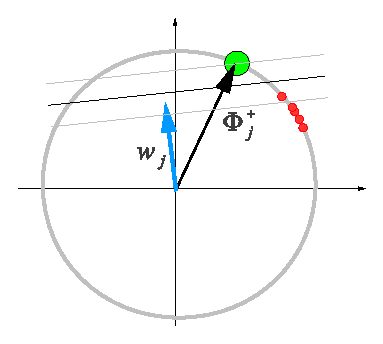
\includegraphics[width=0.45\linewidth]{imgs/figSVM01tight}
                  }
                  %        $C_2 \rightarrow 0$
                  \subfigure[$C_2 \rightarrow 0$]{
                     \centering
                     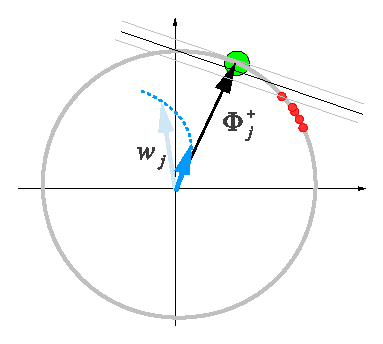
\includegraphics[width=0.45\linewidth]{imgs/figSVM02tight}
                  }
                  \caption{
                     {\bf An illustration of the effect of decreasing parameter $C_2$ in the exemplar support vector machine objective.} 
                     The positive exemplar $\Phi_j^+$ is shown in green. The negative data points are shown in red. All training data is L2 normalized to lie on a hyper-sphere. (a) For $C_2>0$, the normal $w_j$ of the optimal hyper-plane moves away from the direction given by the positive example $\Phi^+$ in a manner that reduces the loss on the negative data.  (b) As the parameter $C_2$ decreases the learnt $w_j$ becomes parallel to the positive training example $\Phi_j^+$ and its magnitude $||w_j||$ goes to 0.
                  }
                  \label{fig:C2effect}
               \end{center}
            \end{figure}
            %
      \paragraph{Case I: $C_2\rightarrow 0$.}
         The goal is to show that when the weight  $C_2$ of the negative data in objective~\eqref{eq:obj} goes towards zero, the resulting hyperplane vector $w_j$ is parallel with the vector of positive training descriptor $\Phi_j^+$. When $w_j$ is normalized to have unit L2 norm the two vectors are identical. First, let us decompose $w$ into parallel and orthogonal part with respect to the positive training data point $\Phi^+$ (in the following we omit index $j$ for brevity), i.e. $w=w^{\perp}+w^{||}$, where $(w^{\perp})^T \Phi^+ = 0$. Next, we observe that when the weight of the negative data diminishes ($C_2\rightarrow 0$), any non-zero component $w^{\perp}$ will increase the value of the objective. As a result, for $C_2\rightarrow 0$ the objective is minimized by $w^{||}$, i.e.\ the optimal $w$ is parallel with $\Phi^+$.

         In detail, for $w=w^{\perp}+w^{||}$, the objective~(\ref{eq:obj}) can be written as
            %
            \begin{align}
               \label{eq:decomposedOrig}
                 ||w^{\perp}+w^{||}||^{2} &+
                 C_1 \cdot h
                 \left(
                  (w^{\perp}+w^{||})^T\Phi^+ + b
                 \right) \\ \nonumber
                 &+
                 C_2\sum_{\Phi\in \mathcal N} h
                 \left(
                  -(w^{\perp}+w^{||})^T\Phi-b
                 \right).
            \end{align}
            %
         Note that the orthogonal part $w^{\perp}$ does not change the value of  the second term in~(\ref{eq:decomposedOrig}) because $(w^{\perp}+w^{||})^T\Phi^+=(w^{||})^T\Phi^+$, and hence~(\ref{eq:decomposedOrig}) reduces to
            %
            \begin{align} 
               \label{eq:decomposed} 
               ||w^{\perp}+w^{||}||^{2} &+
               C_1 \cdot h
               \left(
                   w^{||T}\Phi^+ +b_j
               \right) \\ \nonumber
               &+
               C_2\sum_{\Phi\in \mathcal N} h
               \left(
                   -(w^{\perp}+w^{||})^T\Phi-b
               \right).
            \end{align}
            %
         In the limit case as $C_2 \rightarrow 0$ any non-zero component $w^{\perp}$
         will increase the value of the objective~\eqref{eq:decomposed}. This can be seen by noting that the third term vanishes when $C_2 \rightarrow 0$ and hence the objective is dominated by the first two terms. Further, the second term in~\eqref{eq:decomposed} is independent of $w^{\perp}$. Finally, the first term will always increase for any non-zero value of $w^{\perp}$ as $||w^{\perp}+w^{||}||^{2} \geq ||w^{||}||$ for any $w^{\perp}\neq0$.

         As a result, in the limit case when $C_2 \rightarrow 0$ the optimal $w$ is parallel with $\Phi^+$. Note also, that when $C_2$ is exactly equal to zero, $C_2=0$, the optimal $w$ vanishes, i.e. the objective~\eqref{eq:decomposed} is minimized by trivial solution $||w||=0$ and $b_j=-1$. The effect of decreasing the parameter $C_2$ is illustrated in figure~\ref{fig:C2effect}.


      \paragraph{Case II: $C_2>0$.}
         When the weight $C_2$ of the negative data in the objective~\eqref{eq:decomposed} increases the direction of the optimal $w$ will be different from $w^{||}$ and will change to take into account the loss on the negative data points. Explicitly writing the hinge-loss $h(x) = \max(1-x,0)$ in the last term of~\eqref{eq:decomposed}, we see that $w$ will move in the direction that reduces $\sum_{\Phi\in \mathcal N}\max \left(1+w^T \Phi + b ,0 \right)$, i.e.\ that reduces the dot product $w^T \Phi$ on the negative examples that are active (support vectors).

   \subsection{Interpreting normalized $w$ as a new descriptor} %\vspace{-0.2cm} 
      The above analysis demonstrates that as $C_2$ decreases the normal of the optimal hyperplane $w$ that separates the positive exemplar $\Phi^+$ from negative data becomes parallel with $\Phi^+$, as shown in figure \ref{fig:C2effect}. As $C_2$ increases, the normal $w$ of the optimal hyper-plane moves away from the direction given by the positive example $\Phi^+$ in a manner that reduces the loss on the negative data. 
      This suggests that the learnt $w$ could be interpreted as a modified positive example $\Phi^+$, re-weighted to emphasize directions that separate $\Phi^+$ from the negative data. As discussed above $w$ is not normalized. As we wish to measure the similarity between descriptors by (the cosine of) their angle given by equation \eqref{eq:class}, additional normalization of the learnt $w$ is necessary. Hence we define the new descriptor $\Psi_j$ as the normalized hyperplane normal $w_j$
         %
         \begin{equation}
            \label{eq:normalization}
            \Psi_j=\dfrac{w_j}{||w_j||}.
         \end{equation}
      \textcolor{petr}{%TODO: \emph{we should't speak about calibration, we shoud address not ignoring $b$}\\
%      Measuring the similarity between descriptors by their normalized cross-correlation 
         Note again that for L2 normalized query descriptor $\Phi_q$, evaluating $\Phi_q^T\Psi_j$ in eq.~\eqref{eq:class} corresponds to computing the~normalized cross-correlation between $\Phi_q$ and $\Psi_j$. This was found to work well in retrieval (see e.g.~\cite{Sivic03}) or matching whitened HOG descriptors \cite{Gharbi12, Hariharan12}, but has not yet been used in conjunction with SVMs.    
         Note that while the bias term $b$ is not directly used in the construction of $\Psi_j$, the bias affects the learnt optimal $w_j$ as it appears in the SVM objective~\eqref{eq:obj}. 
         % when learning the optimal SVM hyper-plane $w_j$.           
%         even the new descriptor $\Psi_j$ is obtained by normalization of the learnt hyperplane $w_j$, the bias $b$ form equation~\eqref{eq:decomposed} is not ignored. Indeed, the bias term in convex objective~\eqref{eq:obj} is affecting the learnt the hyperplane.
%         %\\
         %The proposed re-normalization procedure can be interpreted as a simple form of affine calibration where the uncalibrated SVM score $s(x)=w^T x+b$ is transformed into a calibrated score $f(x)=\alpha s(x)+\beta$, where $\alpha = 1/||w||$ and $\beta = -b\alpha$. Note that the bias term b is not ignored but used to compute $f(x)$. The intuition is that for L2 normalized descriptors x computing the calibrated score $f(x)$ corresponds to computing the normalized cross-correlation between vectors w and x. This was found to work well in retrieval (see e.g. Sivic and Zisserman, ICCV 2003 [32]) or matching whitened HOG descriptors [11,13] (see e.g. [Doersch et al., Mid-Level Visual Element Discovery as discriminative Mode Seeking, NIPS 2013]), but has not yet been used in conjunction with SVMs as done in this work. Note also that the affine calibration can be computed offline and does not need any additional computation or storage at query time compared to the p-value calibration of Gronat et al. [12].
      }



\section{Experimental evaluation}
\label{sec:exp}
   In this section we first describe the experimental set-up, then give implementation details, and finally report results of the proposed approach on two datasets where we compare performance with raw Fisher vector matching and several baselines methods. 

   \subsection{Experimental set-up}
      We perform experiments on a database of Google Street View images of Pittsburgh downloaded from the Internet. The data contains panoramas covering roughly an area of $1.3 \times 1.2 \; {\rm km}^2$.       
      Similar to~\cite{Chen11}, for each panorama we generate 12 overlapping perspective views corresponding to two different elevation angles to capture both the street-level scene and the building fa\c{c}ades, resulting in a total of 24 perspective views each with $90^\circ$ FOV and resolution of $960 \times 720$ pixels.
      For evaluation we have used two versions of this data. The first one was obtained from the authors of~\cite{Gronat13} ($25$k images). In the second version we download additional images to increase the dataset size to $55$k images. 
      As a query set with known ground truth GPS positions, we use the 8999 panoramas from the Google Street View research dataset. This dataset covers approximately the same area, but has been captured at a different time, and depicts the same places from different viewpoints and under different illumination conditions. For each test panorama, we generate a set of perspective images as described above. Finally, we randomly select out of all generated perspective views a subset of 4k images, which is used as a test set to evaluate the performance of the proposed approach.
      Since all the query images have associated GPS location we can compute their spatial distance from the database images returned by the matching method. We consider a query image to be correctly localized if the retrieved database image lies within a perimeter of $20m$ from the location of the query.
      %
      \begin{figure}[t!]
         \centering
         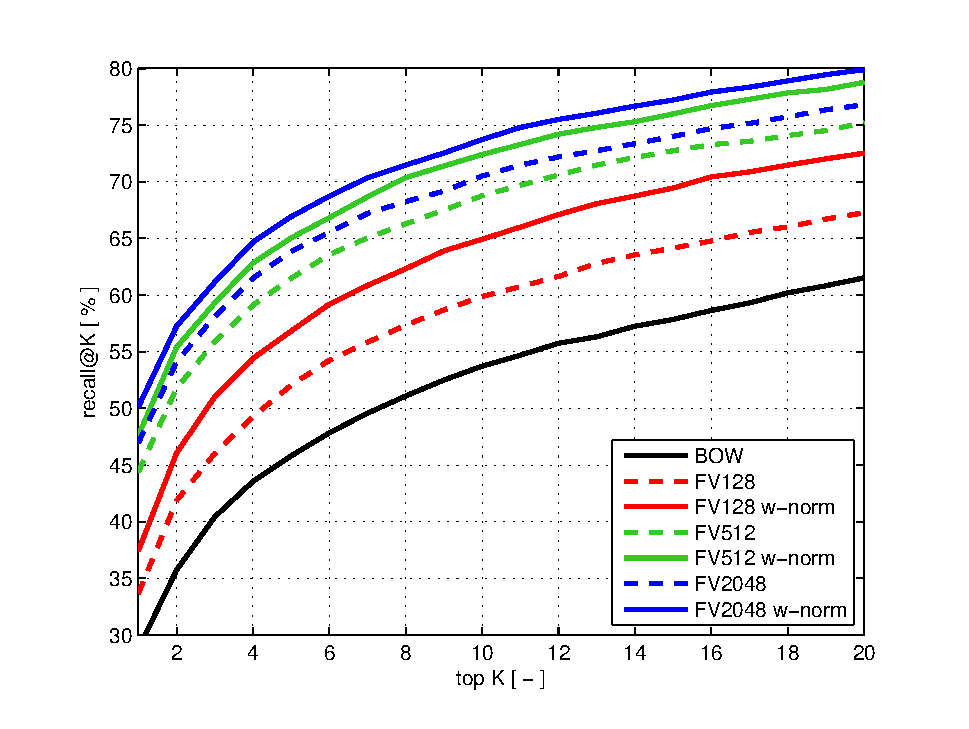
\includegraphics[width=\linewidth]{imgs/plotPitt25kSURF}    
         \caption{
            \textbf{Evaluation on Pittsburgh 25k \cite{Gronat13} dataset.} The fraction of correctly recognized queries (recall@K, y-axis) vs. the number of top $K$ retrieved database images for different Fisher vector dimensions. The learnt descriptors by the proposed method (FV e-SVM) consistently improve over the raw Fisher vector descriptors across the whole range of $K$  and all dimensions.
         }
         \label{fig:recall}
      \end{figure}

   \subsection{Implementation details}
      We first extract rootSIFT descriptors~\cite{Arandjelovic12} for each image. Following~\cite{Jegou12} we project the 128-dimensional SIFT descriptors to 64 dimensions using PCA. The projection matrix is learnt on a set of descriptors from 5,000 randomly selected database images. This has also the effect of decorrelating the SIFT descriptor. 
      The 64-dimensional SIFT descriptors are then aggregated into Fisher vectors using a Gaussian mixture model with $N=256$ components, which  results in a $2\times256\times64 = 32,768$-dimensional descriptor for each image. The Gaussian mixture model is learnt from descriptors extracted from 5,000 randomly sampled database images. 
      The  high-dimensional Fisher vector descriptors are then projected down to dimension $d\in\{128,512, 2048\}$ using PCA learnt from all available images in the database. 
      The resulting low dimensional Fisher vectors are then re-normalized to have unit L2-norm, which we found to be important in practice. 

      \paragraph{Learning parameters and training data.}
         To learn the exemplar support vector machine for each database image $j$, the positive and negative training data are constructed as follows. The \emph{negative training set} $\mathcal N_j$ is obtained by: (i) finding the set of images with geographical distance greater than $200{\rm m}$; (ii)  sorting the images by decreasing value of similarity to image $j$ measured by the dot product between their respective Fisher vectors; (iii) taking the top $N=500$ ranked images as the negative set. In other words, the negative training data consists of the hard negative images, i.e. those that are similar to image $j$ but are far away from its geographical position, hence, cannot have the same visual content. The \emph{positive training set} $\mathcal P_j$
         consist of the original Fisher vector $\Phi_j$ of the image $j$.
         For the SVM training we use {\tt libsvm} \cite{libsvm}.
         We use the same $C_1$ and $C_2$ parameters for all per-exemplar classifiers, but find the optimal value of the parameters for each dimensionality of the Fisher vector by a grid search evaluating performance on a held out set.
         We observe that for different Fisher vector target dimensions the optimal value of parameter $C_1$ is quite stable (typically $C_1=1$) while the optimal parameter for $C_2$ varies between $10^{-6}$ to $10^{-1}$.
         To learn the new image representation for each database image $j$ we: (i) learn SVM from $\mathcal P_j$ and $N_j$ (see above); (ii) $L2$ normalize the learned $w_j$ using equation~\eqref{eq:normalization}; and (iii) use this re-normalized vector as the new image descriptor $\Psi_j$ for image $j$. At query time we compute the Fisher vector $\Phi_q$ of the query image and measure its similarity score to the learnt descriptors $\Psi_j$ for each database image by equation~\eqref{eq:class}.
   

   \subsection{Results} 
      \textcolor{petr}{
         The experiments are performed on two datasets (Pittsburgh 25k and Pittsburgh 55k) on several target Fisher vector dimensions $d\in\{128,512,2048\}$. The proposed approach can be also applied to other descriptors beyond Fisher vectors. To demonstrate this we have applied the proposed method to the bag-of-visual-words (BOW).
         \\
         For each method we measure performance using the percentage of correctly recognized queries (Recall) similarly to, e.g.,~\cite{Chen11,Knopp2010,Sattler-BMVC12}. The query is correctly localized if at least one of the top $K$ retrieved database images is within $20$ meters from the ground truth position of the query. Results are shown for different values of $K$ in tables~\ref{tab:recallBOW},~\ref{tab:recall} and \ref{tab:recall2}. For the Pittsburgh 25k we also show results in the form of a curve in figure~\ref{fig:recall}. The results clearly demonstrate the benefits of the learnt descriptors with respect to the standard Fisher vectors for all target dimensions and lengths of shortlist $K$. The benefits of discriminative learning are specially prominent for low-dimensional compact descriptors ($d=128$). Figure~\ref{fig:images} shows examples of place recognition results.
      }

      % For both databases (Pittsburgh 25k and Pittsburgh 55k) we compare results of our method (FV e-SVM) to two baselines: standard bag-of-visual-words baseline (BOW) and raw Fisher vector matching without learning (FV).  

      % We perform experiments on several target Fisher vector dimensions $d\in\{128,512,2048\}$. For each method we measure performance using the percentage of correctly recognized queries (Recall) similarly to, e.g.,~\cite{Chen11,Knopp2010,Sattler-BMVC12}. The query is correctly localized if at least one of the top $K$ retrieved database images is within $20$ meters from the ground truth position of the query. Results are shown for different values of $K$ in tables~\ref{tab:recall} and \ref{tab:recall2}. For the Pittsburgh 25k we also show results in the form of a curve in figure~\ref{fig:recall}. The results clearly demonstrate the benefits of the learnt descriptors with respect to the standard Fisher vectors for all target dimensions and lengths of shortlist $K$. The benefits of discriminative learning are specially prominent for low-dimensional compact descriptors ($d=128$). 
      % The proposed method also significantly outperforms the bag-of-visual-words baseline. Figure~\ref{fig:images} shows examples of place recognition results. 

      \paragraph{Bag-of-visual-words.}
         \textcolor{petr}{
            For bag of visual words image representation we provide three kind of results summarized in table \ref{tab:recallBOW}. First, similarly to \cite{Gronat13}, we compare the proposed method (e-SVM) to the standard bag-of-visual-words baseline (BOW). We observe improvement from 28.7\% recall@K=1 (BOW) to 31.8\% recall@K=1 (BOW e-SVM). Secondly, the results are also confronted to the p-value calibration of \cite{Gronat13}. The p-value calibration (BOW p-val) gives marginally better results (33.0\% recall@K=1) but at an increased training cost and a significantly higher required memory footprint at query time, which makes the method hard to scale-up to database sizes beyond 200k images. Finally, we investigate the performance of a raw exemplar-SVM (raw e-SVM) with no calibration. As reported in \cite{Gronat13}, we observe that using raw SVM scores directly with no calibration does not perform on BOW. However, this method gives satisfiable good results on Fisher vectors. Details are given next.
         }


         \begin{table}[b]
            \begin{centering}
               
\begin{tabularx}{0.97\linewidth}{|l|c c c c c|}
  \hline 
  \rowcolor{maroon!50}
  Method: & \multicolumn{5}{c|}{25k Pittsburgh}\\
  \hline 
  \hline 
  \rowcolor{maroon!50}
  recall@K [$\%$]         & 1 & 2 & 5 & 10 & 20 \\
  \hline
  \rowcolor{maroon!10}
  BOW                     & 28.7 & 35.7 & 45.8 & 53.7 & 61.5 \\
  \rowcolor{maroon!10}
  BOW raw SVM             & 6.4  &  8.1 & 13.5 & 17.5 & 20.5 \\ 
  \rowcolor{maroon!10}
  BOW e-SVM               & 31.8          &     38.7      & 49.7          & \textbf{60.2} & \textbf{69.4} \\
  \rowcolor{maroon!10}
  BOW p-val               & \textbf{33.0} & \textbf{40.3} & \textbf{50.2} & 58.7 & 66.4 \\
  \hline
  % \rowcolor{maroon!10}
  % FV128                   & 33.6 & 41.8 & 52.0 & 59.8 & 67.7 \\
  % \rowcolor{maroon!10}
  % FV128 raw SVM           & 32.4 & 41.1 & 52.6 & 60.4 & 68.4 \\
  % \rowcolor{maroon!10}
  % \textbf{FV128 e-SVM}    & \textbf{37.8}  & \textbf{46.1} & \textbf{56.9} & \textbf{64.9} & \textbf{72.6}  \\
  % \hline
  % \rowcolor{maroon!10}
  % FV512                 & 44.3 & 51.7 & 61.4 & 68.7 & 75.2 \\
  % \rowcolor{maroon!10}
  % \textbf{FV512 e-SVM}  & \textbf{47.6}  & \textbf{55.4} & \textbf{65.1} & \textbf{72.4} & \textbf{78.8} \\
  % \hline
  % \rowcolor{maroon!10}
  % FV2048        & 46.9    & 54.1 & 63.8 & 70.5 & 76.8 \\
  % \rowcolor{maroon!10}
  % \textbf{FV2048 e-SVM}   & \textbf{50.2} & \textbf{57.3} & \textbf{67.0} & \textbf{73.8} & \textbf{78.0} \\
  % \hline
\end{tabularx}
            \caption{ \textbf{Results on Pittsburgh 25k dataset - BOW.}
                  The fraction of correctly recognized queries (recall@K)
                  \textcolor{petr}{
                     in the top $K\in\{1,2,5,10,20\}$ retrieved images.
                     % Different methods have been applied to two types of descriptors, the BOW and Fisher vectors compressed to different dimensions. The learnt representations (BOW \emph{e-SVM} and BOW \emph{p-val}) outperform the raw BOW baseline as well as the learnt representation without calibration (BOW raw SVM).
                  } 
                  The learnt descriptors by the proposed method (BOW e-SVM) marginally improves over the raw bag-of-visual-words descriptors (BOW).
%                   on both the 25k and 55k Pittsburgh image datasets.     
            }
            \label{tab:recallBOW}
            \end{centering}
         \end{table}

      \paragraph{Fisher vectors.}
         \begin{table}[b]
            \begin{centering}
               
\begin{tabularx}{0.97\linewidth}{|l|c c c c c|}
  \hline 
  \rowcolor{maroon!50}
  Method: & \multicolumn{5}{c|}{25k Pittsburgh}\\
  \hline 
  \hline 
  \rowcolor{maroon!50}
  recall@K [$\%$]         & 1 & 2 & 5 & 10 & 20 \\
  \hline
  \rowcolor{maroon!10}
  BOW                     & 28.7 & 35.7 & 45.8 & 53.7 & 61.5 \\
  \rowcolor{maroon!10}
  BOW raw SVM             & 6.4  &  8.1 & 13.5 & 17.5 & 20.5 \\ 
  \rowcolor{maroon!10}
  BOW e-SVM               & 31.8 & 38.7 & 49.7 & 60.2 & 69.4 \\
  \rowcolor{maroon!10}
  BOW p-val               & 33.0 & 40.3 & 50.2 & 58.7 & 66.4 \\
  \hline
  \rowcolor{maroon!10}
  FV128                   & 33.6 & 41.8 & 52.0 & 59.8 & 67.7 \\
  \rowcolor{maroon!10}
  FV128 raw SVM           & 32.4 & 41.1 & 52.6 & 60.4 & 68.4 \\
  \rowcolor{maroon!10}
  \textbf{FV128 e-SVM}    & \textbf{37.8}  & \textbf{46.1} & \textbf{56.9} & \textbf{64.9} & \textbf{72.6}  \\
  \hline
  \rowcolor{maroon!10}
  FV512                 & 44.3 & 51.7 & 61.4 & 68.7 & 75.2 \\
  \rowcolor{maroon!10}
  \textbf{FV512 e-SVM}  & \textbf{47.6}  & \textbf{55.4} & \textbf{65.1} & \textbf{72.4} & \textbf{78.8} \\
  \hline
  \rowcolor{maroon!10}
  FV2048        & 46.9    & 54.1 & 63.8 & 70.5 & 76.8 \\
  \rowcolor{maroon!10}
  \textbf{FV2048 e-SVM}   & \textbf{50.2} & \textbf{57.3} & \textbf{67.0} & \textbf{73.8} & \textbf{78.0} \\
  \hline
\end{tabularx}
            \caption{ \textbf{Results on Pittsburgh 25k dataset.}
                  The fraction of correctly recognized queries (recall@K)
                  \textcolor{petr}{
                     in the top $K\in\{1,2,5,10,20\}$ retrieved images.
                     % Different methods have been applied to two types of descriptors, the BOW and Fisher vectors compressed to different dimensions. The learnt representations (BOW \emph{e-SVM} and BOW \emph{p-val}) outperform the raw BOW baseline as well as the learnt representation without calibration (BOW raw SVM).
                  } 
                  The learnt descriptors by the proposed method (FV e-SVM) consistently improve over the raw Fisher vector descriptors (FV) across the whole range of $K$  and all dimensions.
%                   on both the 25k and 55k Pittsburgh image datasets.     
            }
            \label{tab:recall}
            \end{centering}
         \end{table}
         %
         \textcolor{petr}{
         Table \ref{tab:recall} summarizes the results of proposed method that has been applied on Fisher vectors for several target dimensions $d\in\{128,512,2048\}$. The learnt image representation (FV e-SVM) significantly outperforms the Fisher vector baseline (FV). The improvements are consistent across different lengths $K$ of the shortlist for all target dimensions of the Fisher vectors.
         Figure \ref{fig:recall} shows the results in a form of curve and it clearly demonstrates the benefits of the learnt descriptors. For comprehensiveness the figure also shows the BOW baseline curve taken from table \ref{tab:recallBOW} shown in black.
         \\
         The p-val calibration of~\cite{Gronat13} has been also tested on e-SVM Fisher vectors. We found that the calibration did not perform well for the learnt Fisher vector classifiers (top 1 recall of 25.3\% compared to baseline performance of 33.6\% for dimension 128). When examining the results, we believe this may be attributed to the fact that Fisher vectors are low dimensional compared to the extremely high-dimensional (d=100,000) bag-of-visual-words representation, which affects the distribution of the classifier scores on the negative test data.
         \\
         Next, we investigate the performance of a raw exemplar-SVM (raw e-SVM) without any further calibration on Fisher vectors. We observe that while using raw SVM scores directly without any calibration fails for the bag-of-visual-words representation (BOW raw SVM, talbe~\ref{tab:recallBOW}), as reported in \cite{Gronat13}, it marginally improves the recall for larger $K$ for Fisher vectors (68.4\% for FV128 raw SVM compared to 67.7\% for non-learned FV128).
         \\
         Finally, we performed experiments on the larger Pittsburgh 55k dataset. Similarly to the former dataset, the results summarized in table \ref{tab:recall2} show consistent improvement of the proposed method (FV e-SVM) over the Fisher vector baseline (FV) across all target dimensions. The benefits of the proposed method in terms of memory efficiency will be discussed next.
         }
         %
         \begin{table}[t]
            \begin{centering}
               \begin{tabularx}{0.955\linewidth}{|l|c c c c c|}
	\hline 
	\rowcolor{maroon!50}
	Method: & \multicolumn{5}{c|}{55k Pittsburgh} \\
	\hline 
	\hline 
	\rowcolor{maroon!50}
	recall@K [$\%$] 			& 1 & 2 & 5 & 10 & 20 \\
	\hline
	\rowcolor{maroon!10}
	BOW         				& 8.7 & 11.0 & 17.3 & 22.8 & 25.4  \\
	\hline
	\rowcolor{maroon!10}
	FV128         				& 10.9 & 14.1 & 20.2 & 26.4 & 33.2 \\
	\rowcolor{maroon!10}
	\textbf{FV128 e-SVM} 		& \textbf{13.5}  &  \textbf{17.7}  &  \textbf{25.0}  &  \textbf{31.8}  &  \textbf{39.0} \\
	\hline
	\rowcolor{maroon!10}
	FV512         				& 17.3 &  21.1 &  28.4 &  34.2 &  40.3 \\
	\rowcolor{maroon!10}
	\textbf{FV512 e-SVM}   		& \textbf{19.8} &  \textbf{25.1} &  \textbf{32.7}  & \textbf{38.7} &  \textbf{46.0} \\
	\hline
	\rowcolor{maroon!10}
	FV2048        				& 19.2 & 23.5 & 29.9 &  35.2 &  41.9 \\
	\rowcolor{maroon!10}
	\textbf{FV2048 e-SVM}  		& \textbf{20.8} & \textbf{25.9} & \textbf{33.1} & \textbf{38.7} & \textbf{45.9} \\
	\hline
\end{tabularx}
               \caption{ \textbf{Results on Pittsburgh 55k dataset - FV.}
                  The fraction of correctly recognized queries (recall@K)
                  \textcolor{petr}{
                  in top $K\in\{1,2,5,10,20\}$ retrieved images.
                  The proposed method (\emph{e-SVM}) has been applied to Fisher vectors compressed to different dimensions.
                  } 
                  The learnt descriptors by the proposed method (FV e-SVM) consistently improve over the raw Fisher vector descriptors across the whole range of $K$  and all dimensions.
%                   on both the 25k and 55k Pittsburgh image datasets.     
               }
            \label{tab:recall2}
            \end{centering}
         \end{table}

      % \paragraph{Applying our learning method to other descriptors.}
      %   \textcolor{petr}{ 
      %    The proposed approach can be applied to other descriptors beyond Fisher vectors. To demonstrate this we have applied the proposed method to the bag-of-visual-words descriptor and observed improvement from 28.7\% recall@K=1 (BOW) to 31.8\% recall@K=1 (BOW e-SVM).  
      %    For bag-of-visual-words,  the e-SVM with p-value calibration of~\cite{Gronat13} (BOW p-val) gives a slightly better results (33.6\% recall@K=1) but at an increased training cost and a significantly higher required memory footprint at query time, which makes the method hard to scale-up to database sizes beyond 200k images. The results are given in table \ref{tab:recall} (top four rows).
      %   }

%       \paragraph{Comparison to other methods.}
%          %On the Pittsburgh 25k database, we compare performance of our learnt discriminative descriptors to the methods of~\cite{Gronat13} and~\cite{Knopp2010}, who report on the same testing data top $K=1$ recall of 36.5\% and 41.9\%, respectively (results taken from~\cite{Gronat13}). Our method outperforms~\cite{Knopp2010} already for dimension $d=128$ (37.8\%) and~\cite{Gronat13} for dimension $d=512$ (47.6\%). Furthermore, note that~\cite{Gronat13,Knopp2010} are based on a bag-of-visual-words representation, which typically needs to store between 1000-2000 non-zero visual words per image, which is significantly more than our learnt 128 or 512 dimensional descriptor. 
%          \textcolor{petr}{
%          On the Pittsburgh 25k database, we compare performance of our learnt discriminative descriptors to the method of~\cite{Gronat13} who report results on similar testing data. Our method outperforms~\cite{Gronat13} already for dimension $d=128$ (37.8\%).
%   %       \\
%          We have also tested the p-val calibration of~\cite{Gronat13} on e-SVM Fisher vectors. We found that the calibration did not perform well for the learnt Fisher vector classifiers (top 1 recall of 25.3\% compared to baseline performance of 33.6\% for dimension 128). When examining the results, we believe this may be attributed to the fact that Fisher vectors are low dimensional compared to the extremely high-dimensional (d=100,000) bag-of-visual-words representation, which affects the distribution of the classifier scores on the negative test data.
% %         \\
%          Finally, we investigate the performance of a raw exemplar-SVM (raw e-SVM) without any further calibration for both image descriptors . We observe that while using raw SVM scores directly without any calibration fails for the bag-of-visual-words representation (BOW raw SVM) (as reported in \cite{Gronat13}), it marginally improves recall for larger $K$ for Fisher vectors (68.4\% for FV128 raw SVM compared to 67.7\% for non-learned FV128).
% %         as indicated in \ref{tab:recall} (FV128 raw SVM).
%           %We have compared the proposed method with the p-value calibration of (Gronat et al.[12]) applied to Fisher vectors. The results show that our method significantly outperforms the p-value calibration (37.8\% recall@1 vs. 32.3\% recall@1; 56.9\%recall@5 vs. 50.0\% recall@5) for the Fisher vector of dimension 128. Similar gains are observed for other FV dimensions.
%         }
      \paragraph{Memory complexity analysis.}
         Figure~\ref{fig:memory} compares the performance of the learnt discriminative descriptor (FV eSVM) to the raw Fisher vectors (FV) for different target dimensions. 
         The results demonstrate that for a given level of accuracy (y-axis) our method learns a more compact (lower-dimensional) representation (x-axis). For example, our learnt 128-dimensional descriptor achieves a similar accuracy (around 65\%) to the 256-dimensional raw Fisher descriptor essentially reducing the memory complexity to 50\% for the same level of performance.  Note that 
         similar to~\cite{Jegou12}, we observe decrease in performance at high-dimensions for both the baseline and our method.
         %
         \begin{figure}[t!]
            \centering
            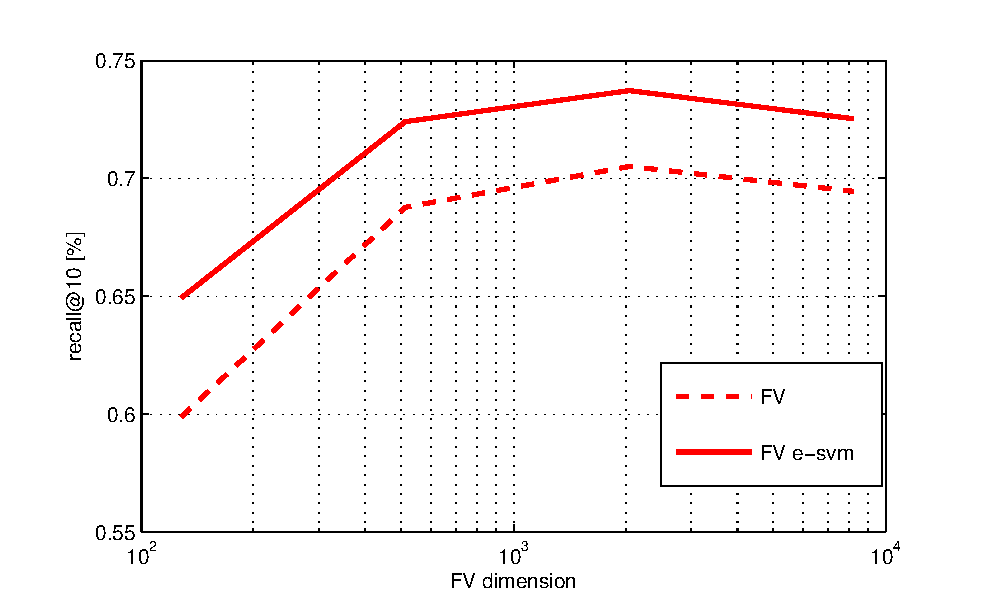
\includegraphics[width=1.0\linewidth]{imgs/FVmemory}    
            \caption{
               \textbf{Memory complexity analysis.} 
               The fraction of correctly localized queries at the top 10 retrieved images (y-axis) for different Fisher vector dimensions (x-axis). The learnt descriptors by our method (FV e-SVM) clearly outperform the raw Fisher vector descriptors (FV) for all dimensions. Note that for a certain level of performance (y-axis) the proposed method learns a more memory efficient (lower dimensional, x-axis) descriptor.
            }
            \label{fig:memory}
         \end{figure}
         %
         %
         %
         %
         %
         \begin{figure*}[h]
                    %%%%%%%%%%% Example 1 %%%%%%%%%%%%%%%
        \begin{minipage}{1.0\linewidth}
        \end{minipage}
        % QUERY image
        \begin{minipage}{0.34\linewidth}
            \centering
            \vspace{0mm}
            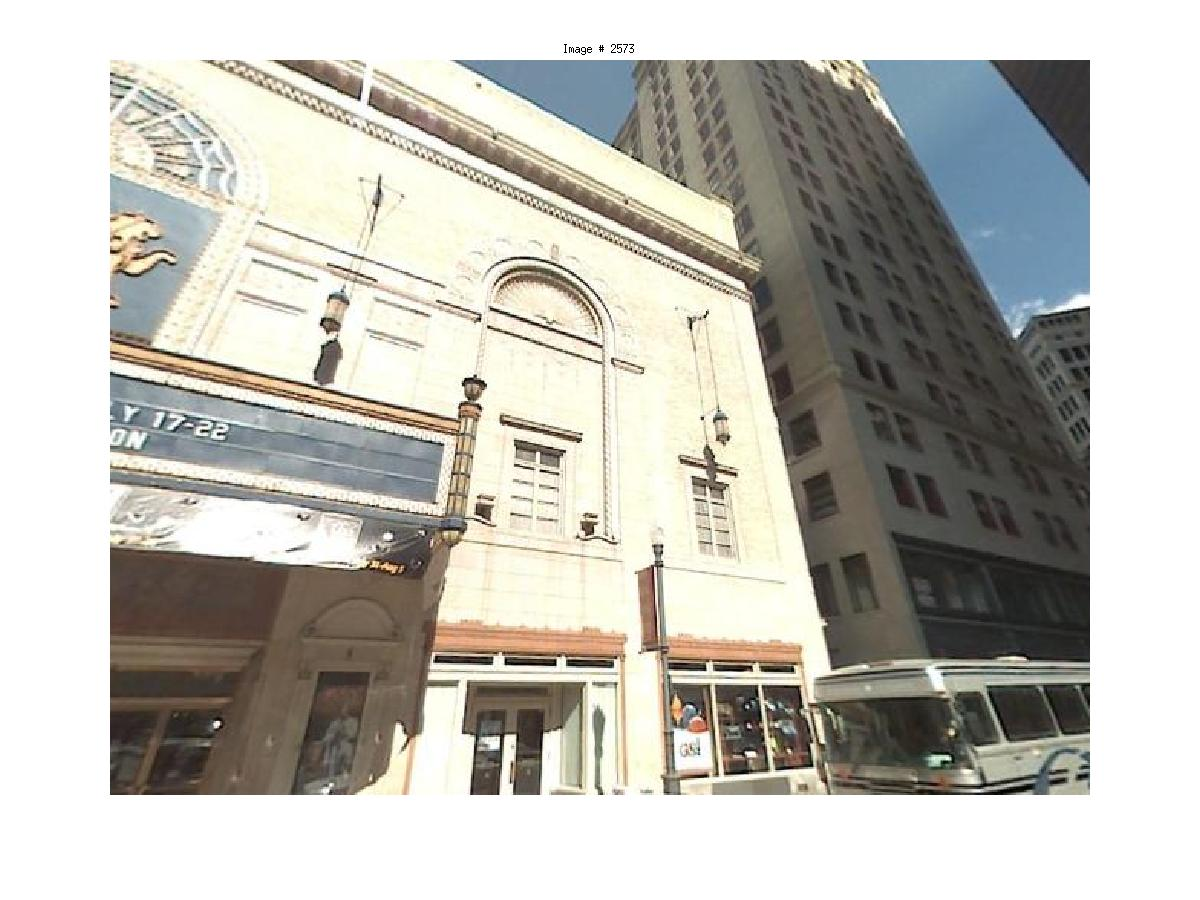
\includegraphics[trim = 45mm 40mm 45mm 30mm, clip=true,height=36mm]{imgs/Wnorm/exImproved02/query.jpg}
        \end{minipage}
        % Retrieved images
        \begin{minipage}{0.75\linewidth}
            % FV e-SVM
            \begin{minipage}{\linewidth} 
                \colorbox{myGreen}{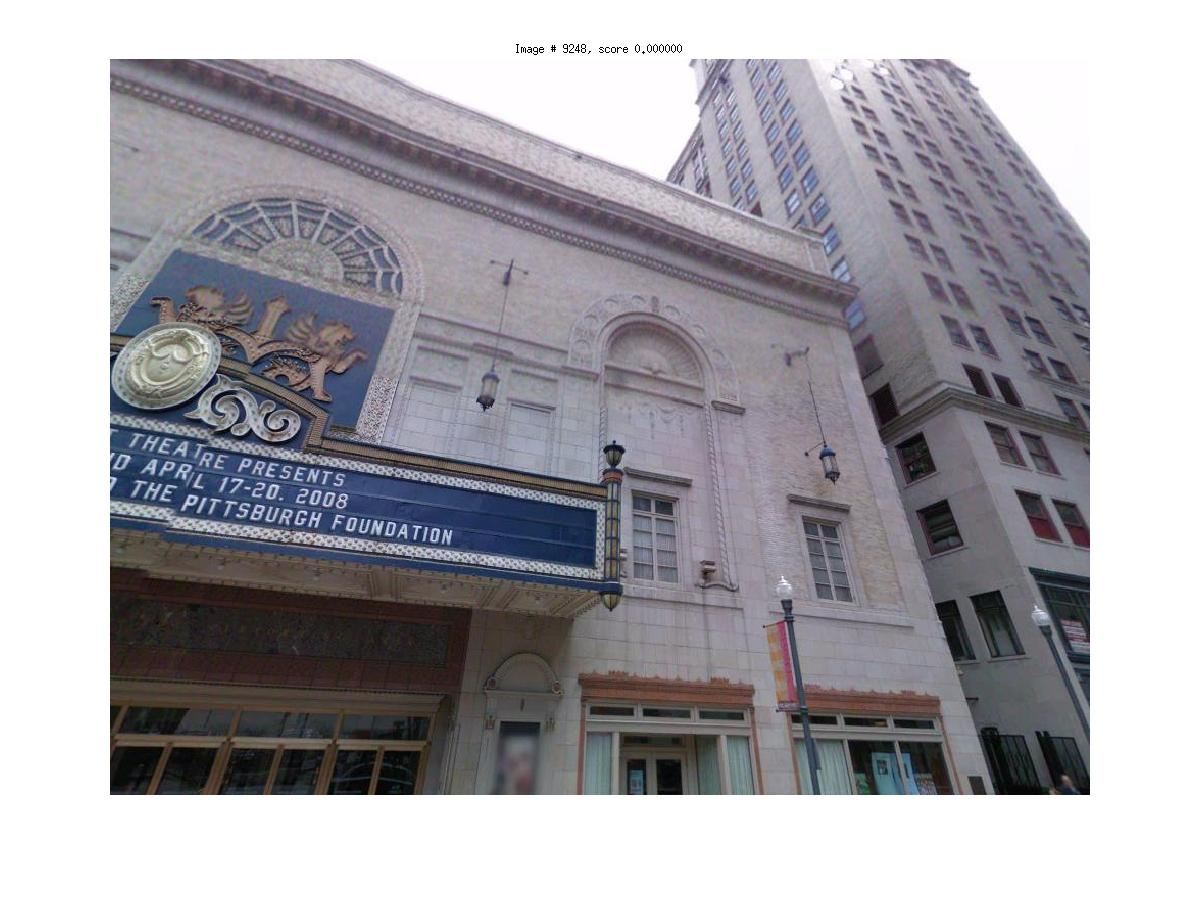
\includegraphics[trim = 35mm 30mm 35mm 30mm, clip=true, height=16mm]{imgs/Wnorm/exImproved02/improvedPval01.jpg}}
                \colorbox{myGreen}{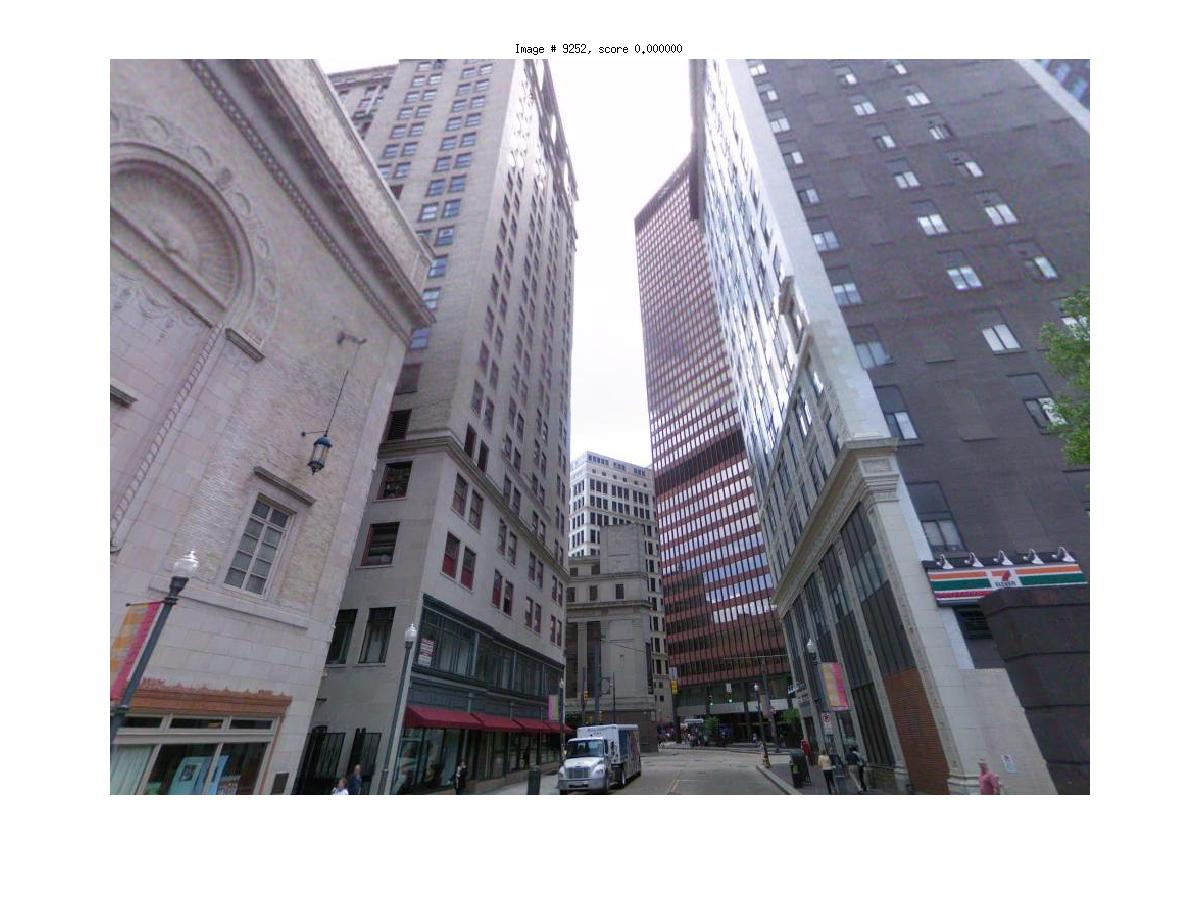
\includegraphics[trim = 35mm 30mm 35mm 30mm, clip=true, height=16mm]{imgs/Wnorm/exImproved02/improvedPval02.jpg}}
                \colorbox{myGreen}{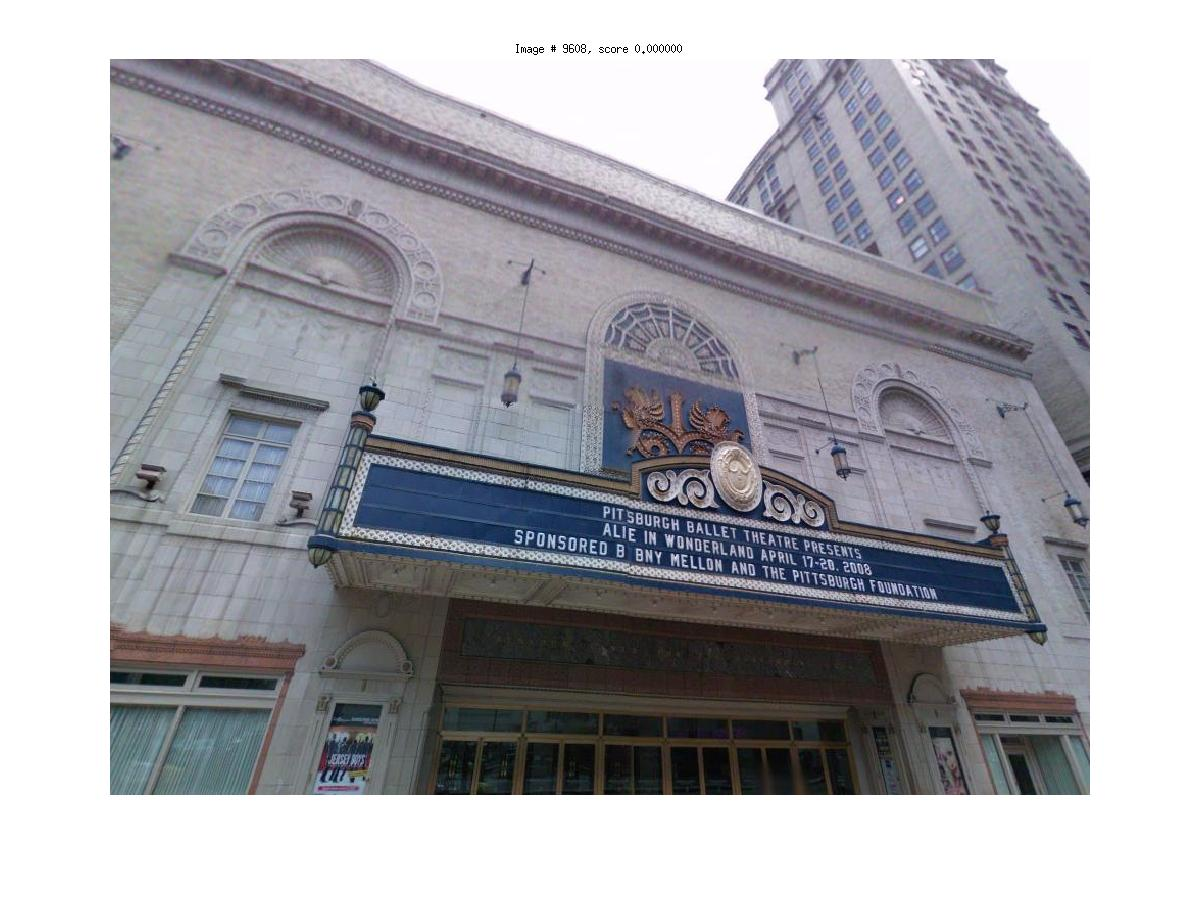
\includegraphics[trim = 35mm 30mm 35mm 30mm, clip=true, height=16mm]{imgs/Wnorm/exImproved02/improvedPval03.jpg}}
                \colorbox{myGreen}{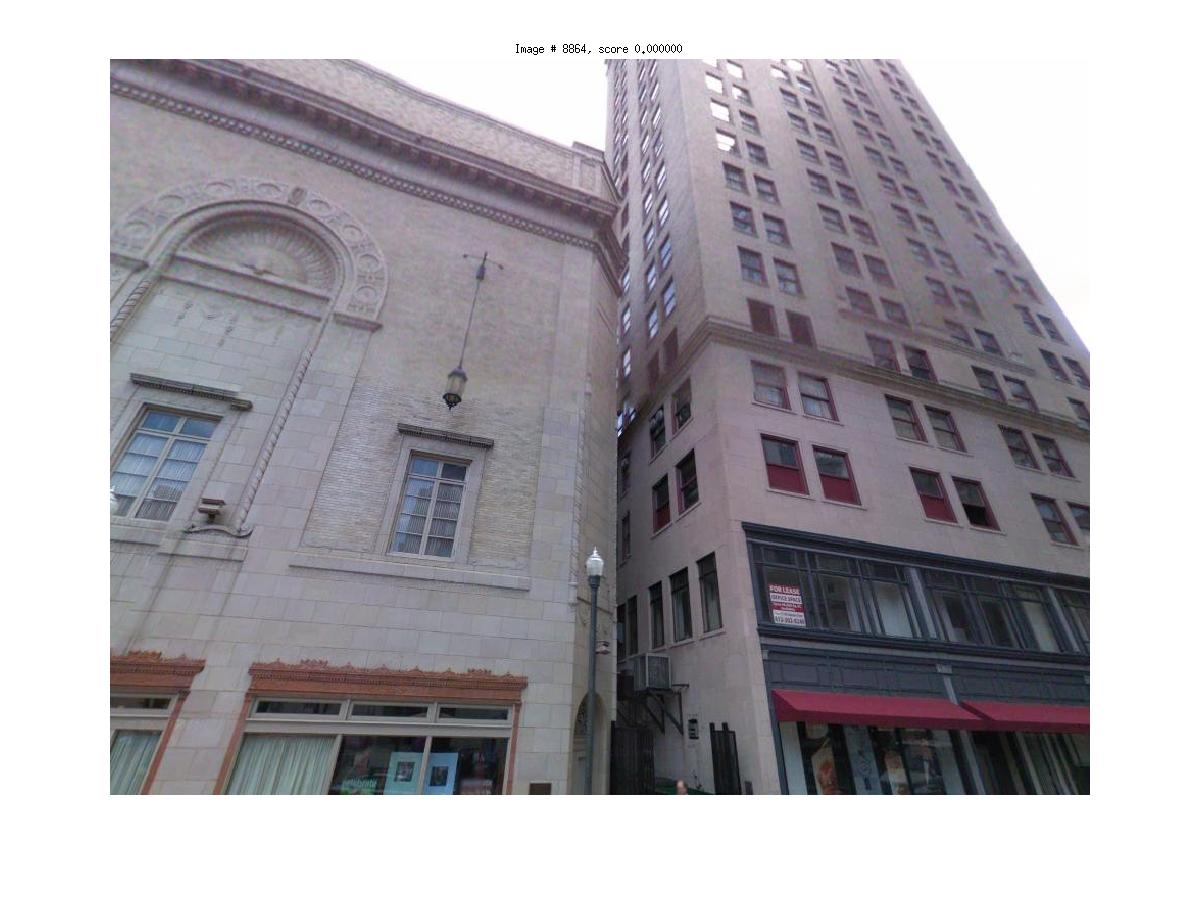
\includegraphics[trim = 35mm 30mm 35mm 30mm, clip=true, height=16mm]{imgs/Wnorm/exImproved02/improvedPval04.jpg}}
            \end{minipage}
            \\
            \begin{minipage}{\linewidth}
                \colorbox{myRed}{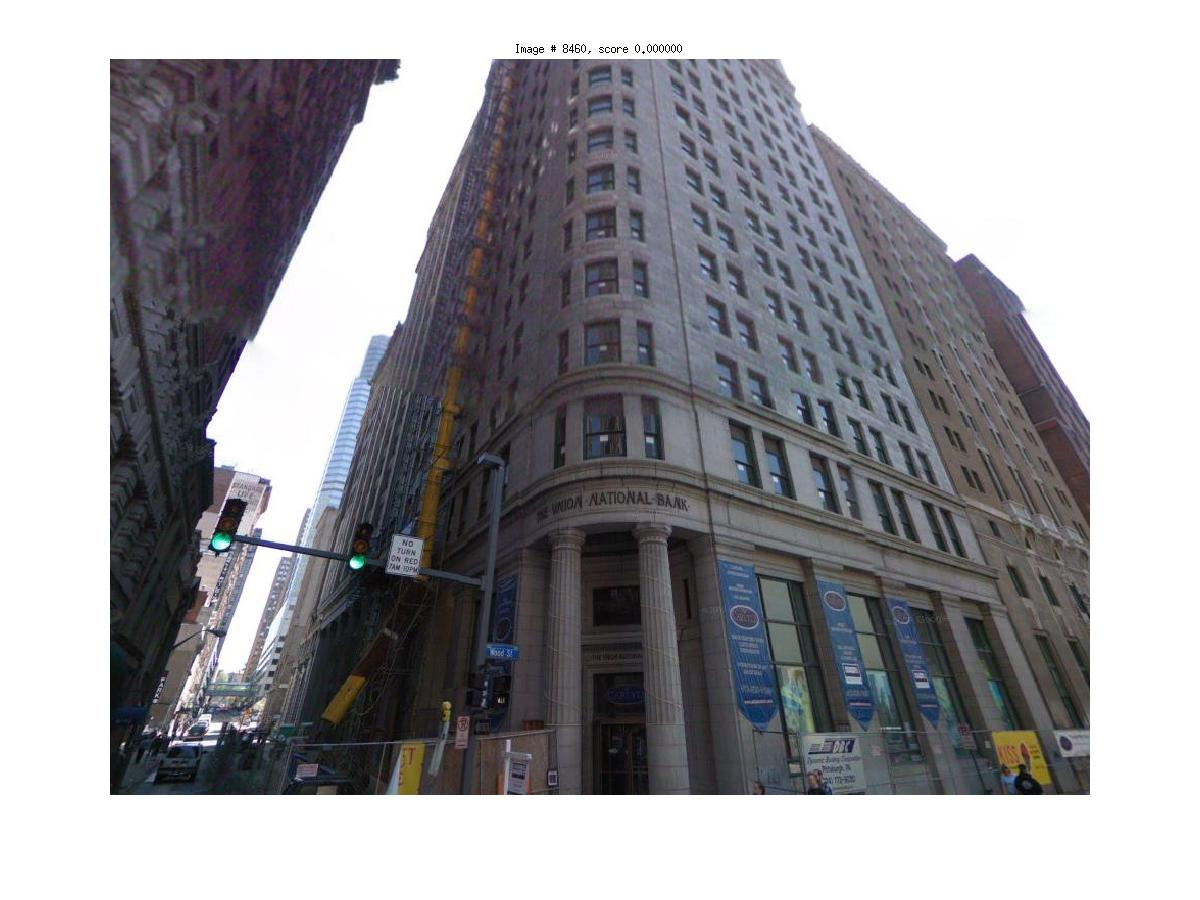
\includegraphics[trim = 35mm 30mm 35mm 30mm, clip=true, height=16mm]{imgs/Wnorm/exImproved02/improved01.jpg}}
                \colorbox{myRed}{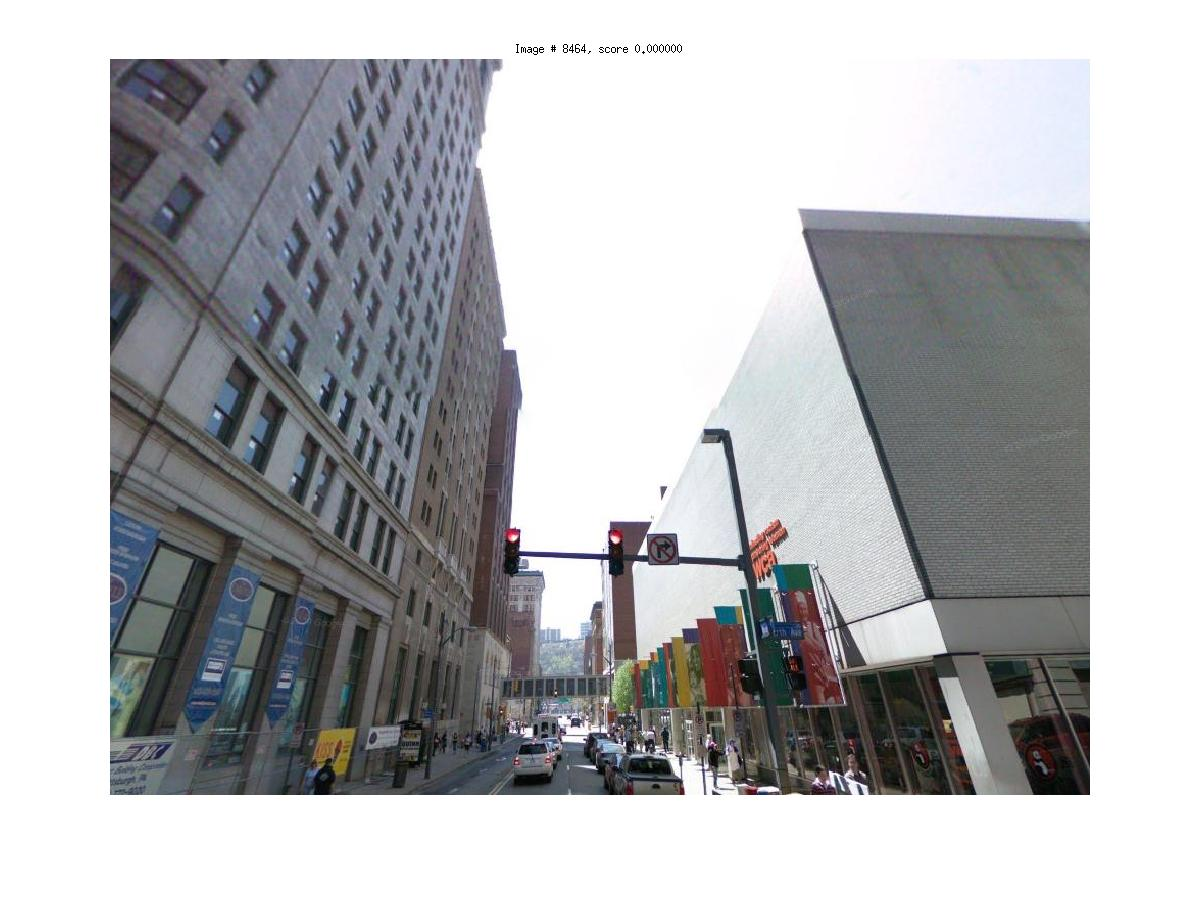
\includegraphics[trim = 35mm 30mm 35mm 30mm, clip=true, height=16mm]{imgs/Wnorm/exImproved02/improved02.jpg}}
                \colorbox{myRed}{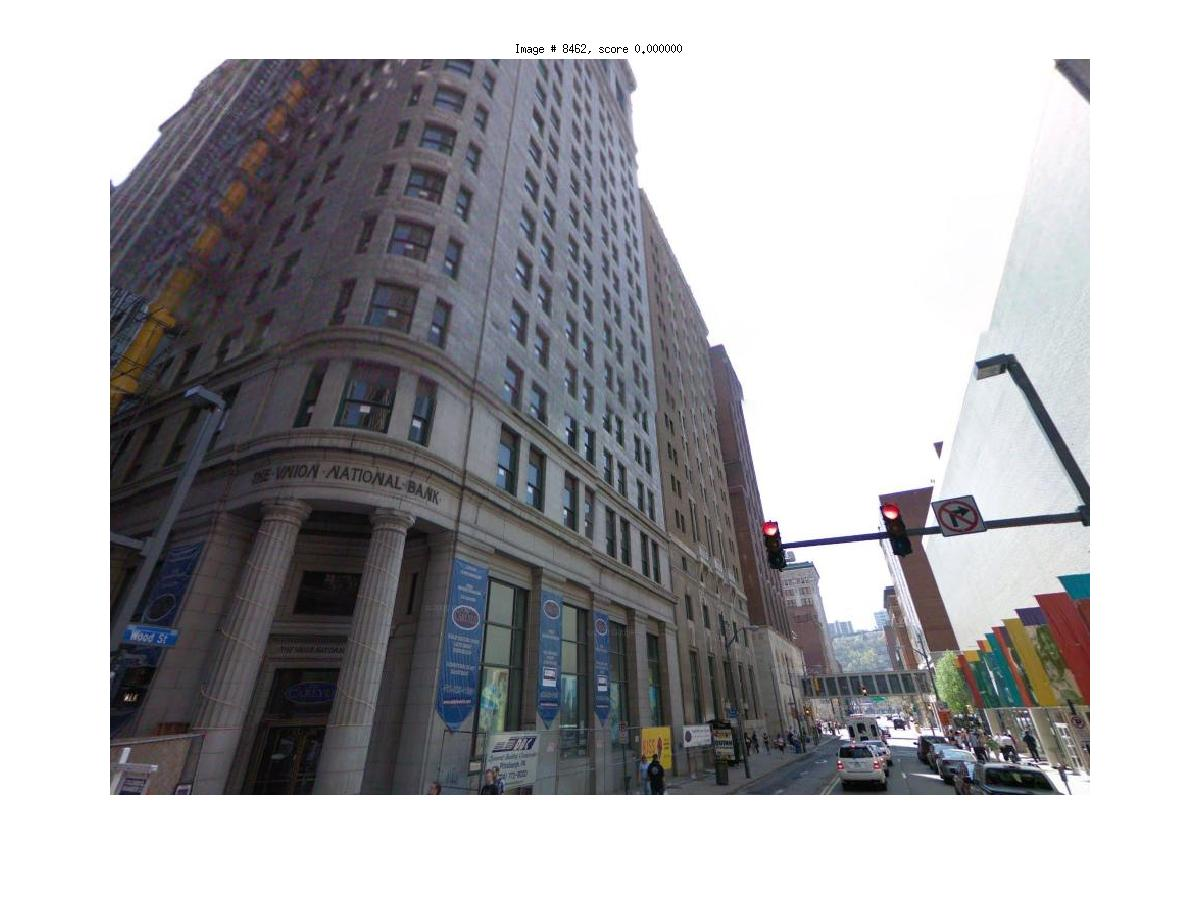
\includegraphics[trim = 35mm 30mm 35mm 30mm, clip=true, height=16mm]{imgs/Wnorm/exImproved02/improved03.jpg}}
                \colorbox{myRed}{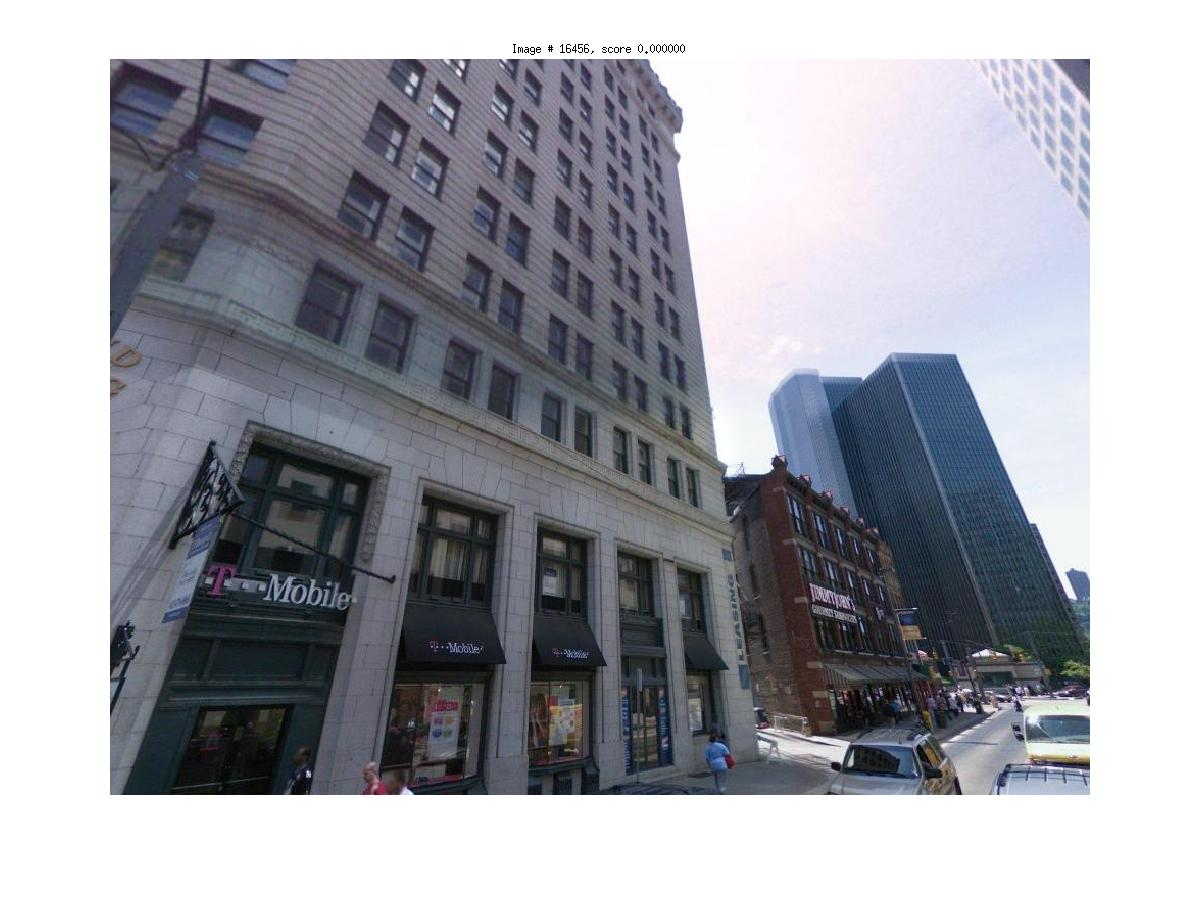
\includegraphics[trim = 35mm 30mm 35mm 30mm, clip=true, height=16mm]{imgs/Wnorm/exImproved02/improved04.jpg}}
            \end{minipage} 
        \end{minipage}
        \vspace{3mm}
        \\
        %%%%%%%%%%% Example 2 %%%%%%%%%%%%%%%
        \begin{minipage}{1.0\linewidth}
        \end{minipage}
        % QUERY image
        \begin{minipage}{0.34\linewidth}
            \centering
            \vspace{0mm}
            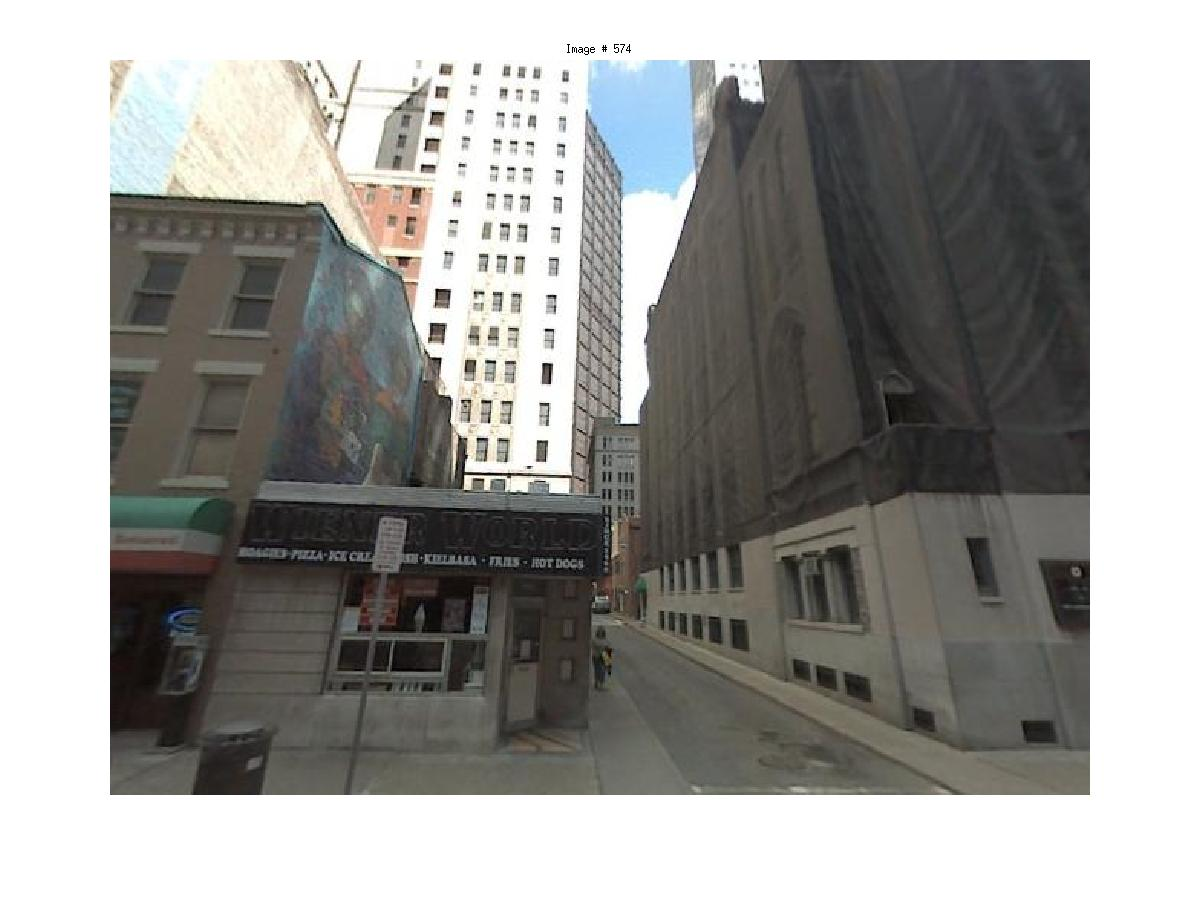
\includegraphics[trim = 45mm 40mm 45mm 30mm, clip=true,height=36mm]{imgs/Wnorm/exImproved05/query.jpg}
        \end{minipage}
        % Retrieved images
        \begin{minipage}{0.75\linewidth}
            % FV e-SVM
            \begin{minipage}{\linewidth} 
                \colorbox{myGreen}{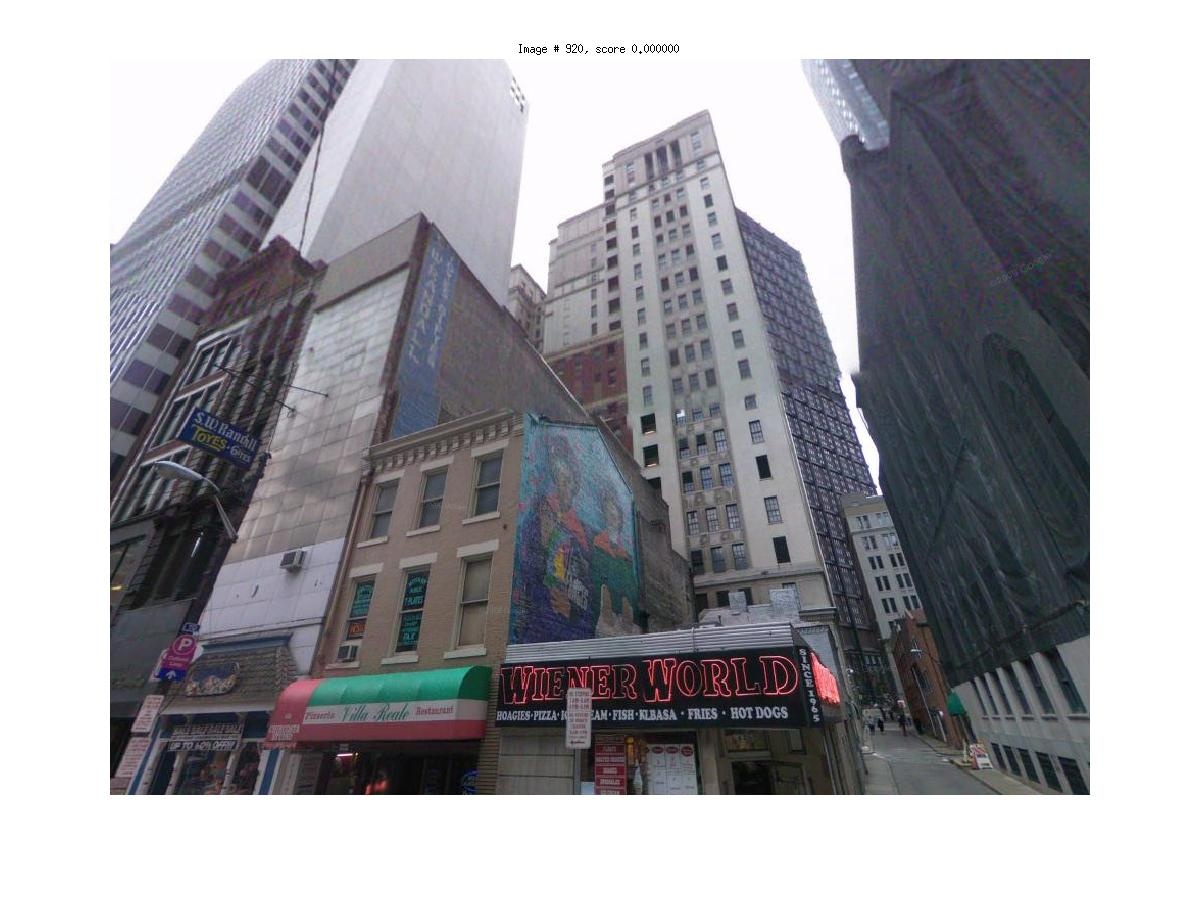
\includegraphics[trim = 35mm 30mm 35mm 30mm, clip=true, height=16mm]{imgs/Wnorm/exImproved05/improvedPval01.jpg}}
                \colorbox{myGreen}{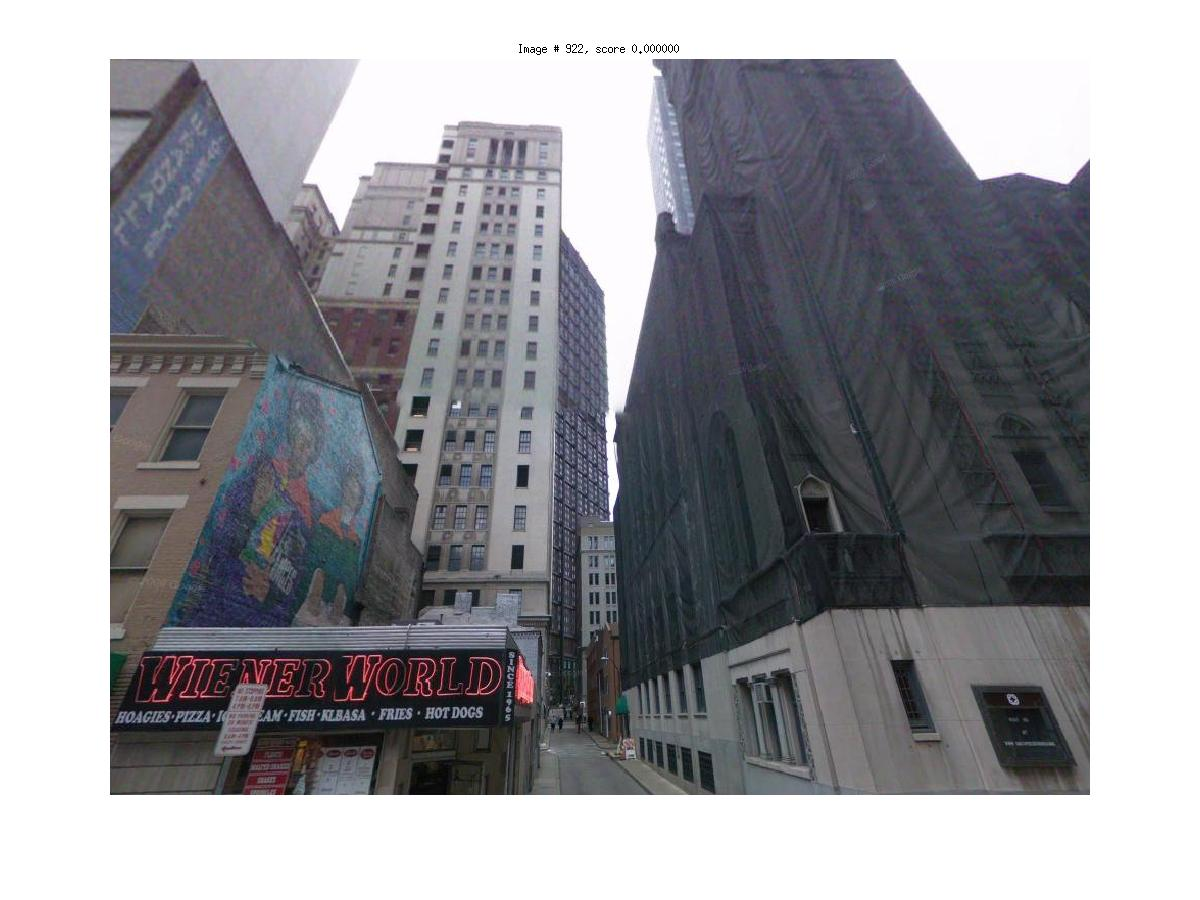
\includegraphics[trim = 35mm 30mm 35mm 30mm, clip=true, height=16mm]{imgs/Wnorm/exImproved05/improvedPval02.jpg}}
                \colorbox{myGreen}{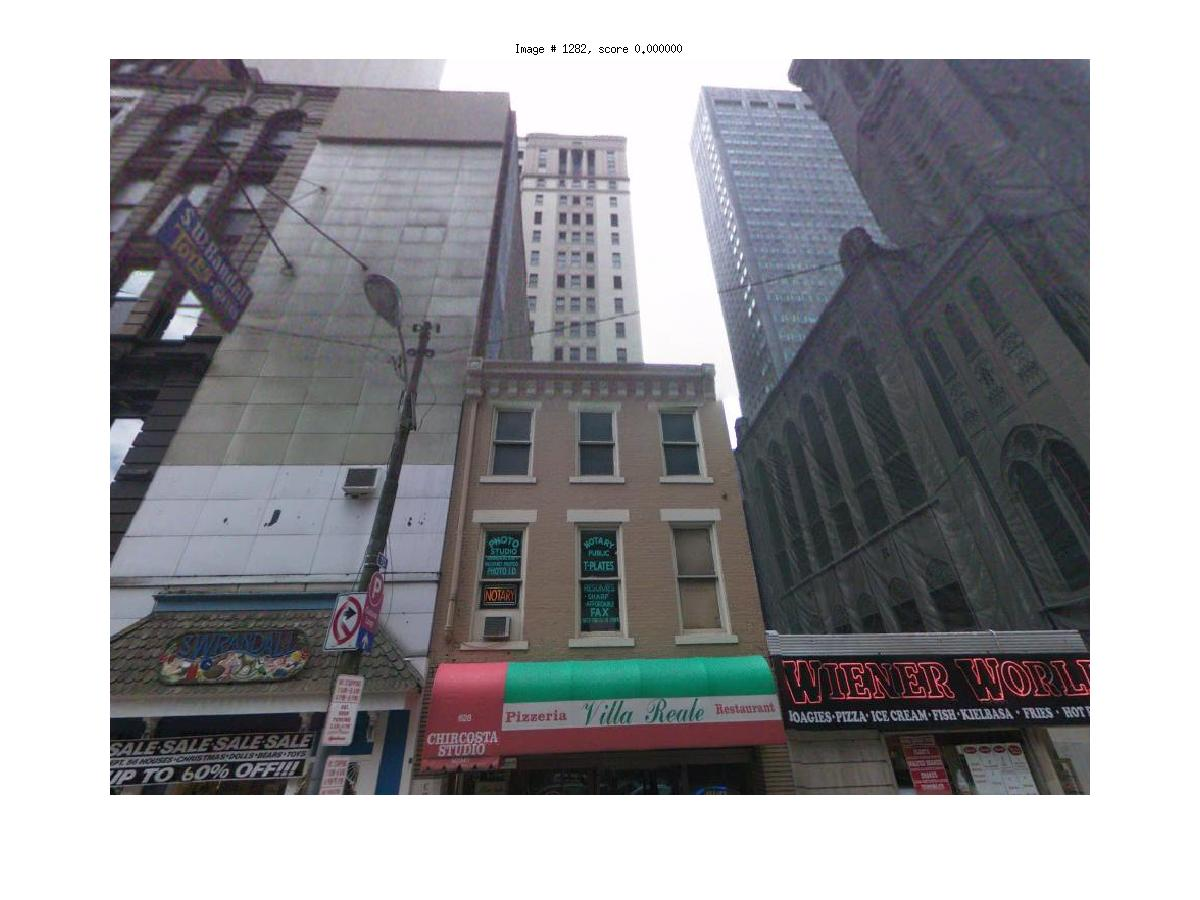
\includegraphics[trim = 35mm 30mm 35mm 30mm, clip=true, height=16mm]{imgs/Wnorm/exImproved05/improvedPval03.jpg}}
                \colorbox{myGreen}{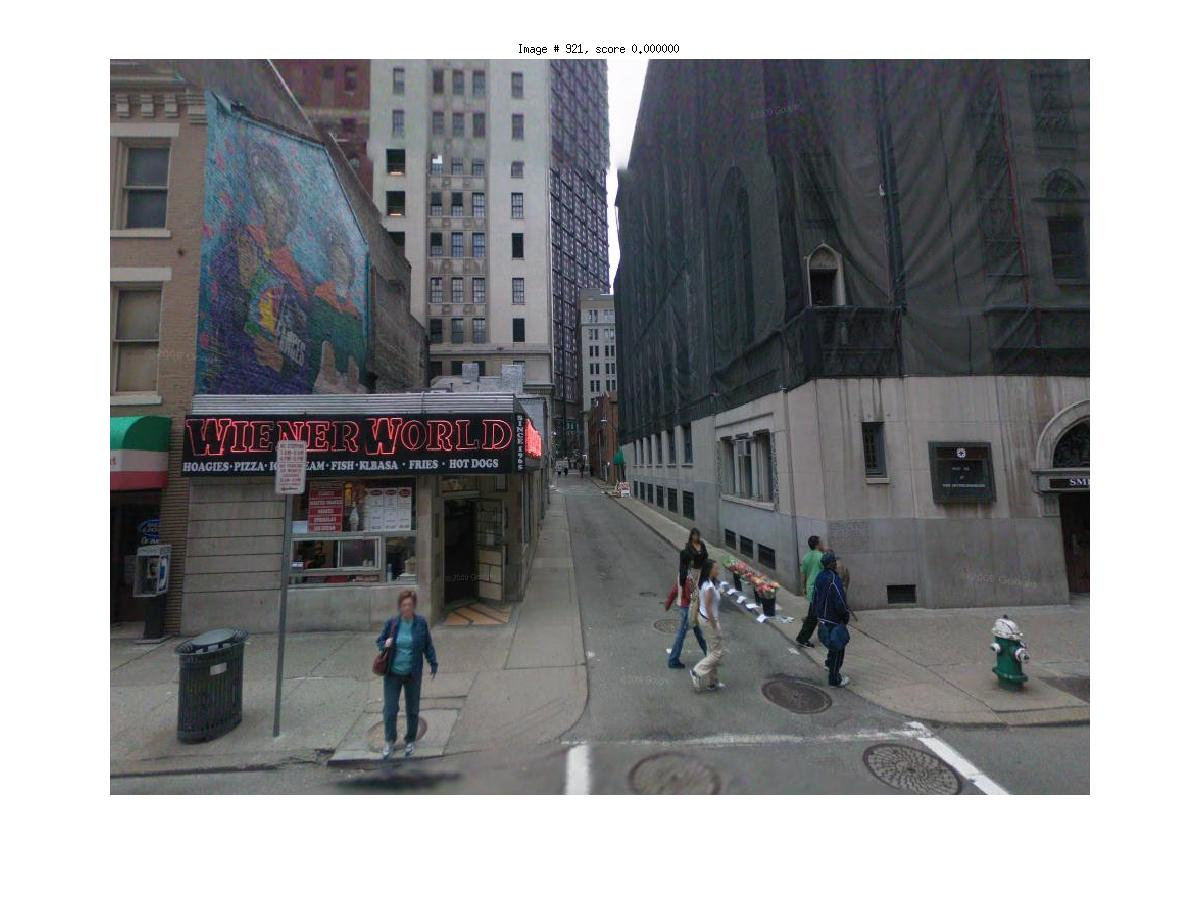
\includegraphics[trim = 35mm 30mm 35mm 30mm, clip=true, height=16mm]{imgs/Wnorm/exImproved05/improvedPval04.jpg}}
            \end{minipage}
            \\
            \begin{minipage}{\linewidth}
                \colorbox{myRed}{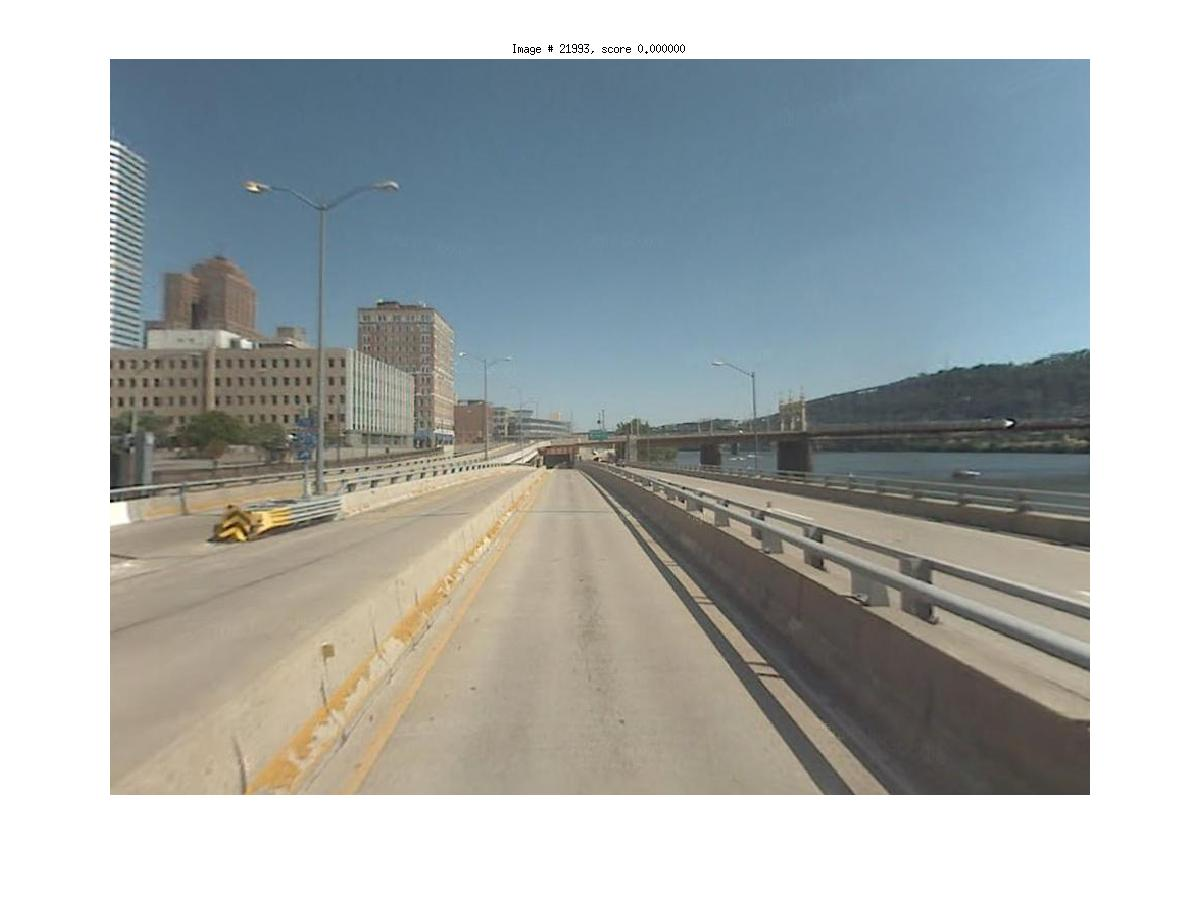
\includegraphics[trim = 35mm 30mm 35mm 30mm, clip=true, height=16mm]{imgs/Wnorm/exImproved05/improved01.jpg}}
                \colorbox{myGreen}{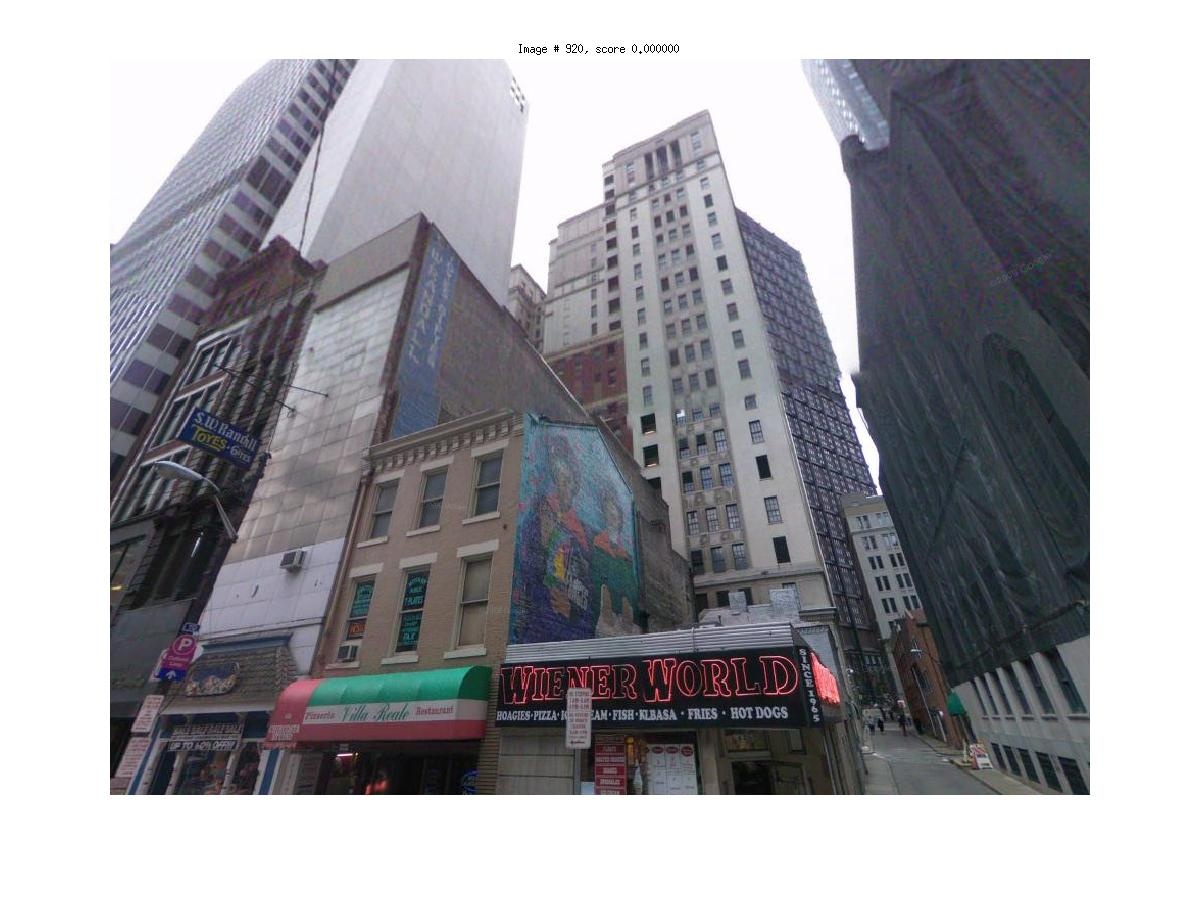
\includegraphics[trim = 35mm 30mm 35mm 30mm, clip=true, height=16mm]{imgs/Wnorm/exImproved05/improved02.jpg}}
                \colorbox{myRed}{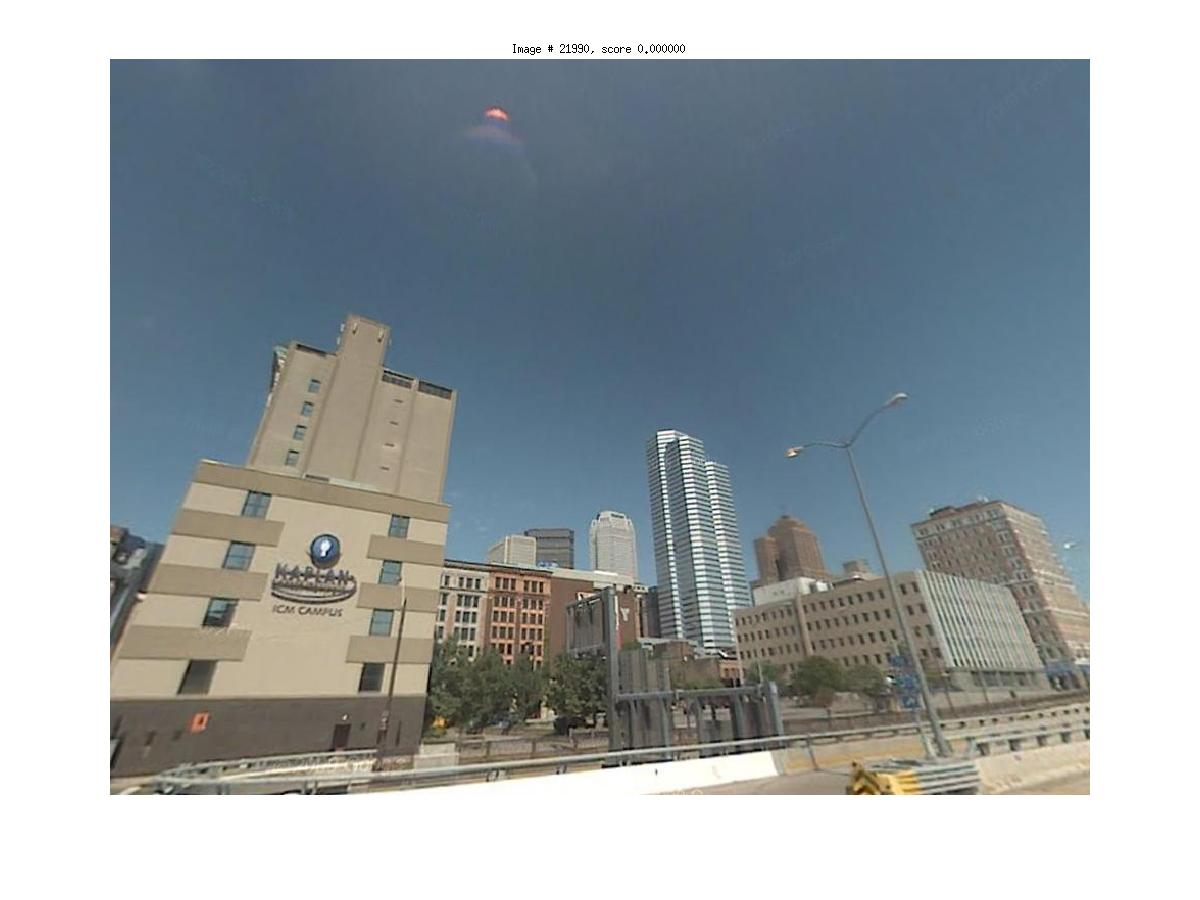
\includegraphics[trim = 35mm 30mm 35mm 30mm, clip=true, height=16mm]{imgs/Wnorm/exImproved05/improved03.jpg}}
                \colorbox{myRed}{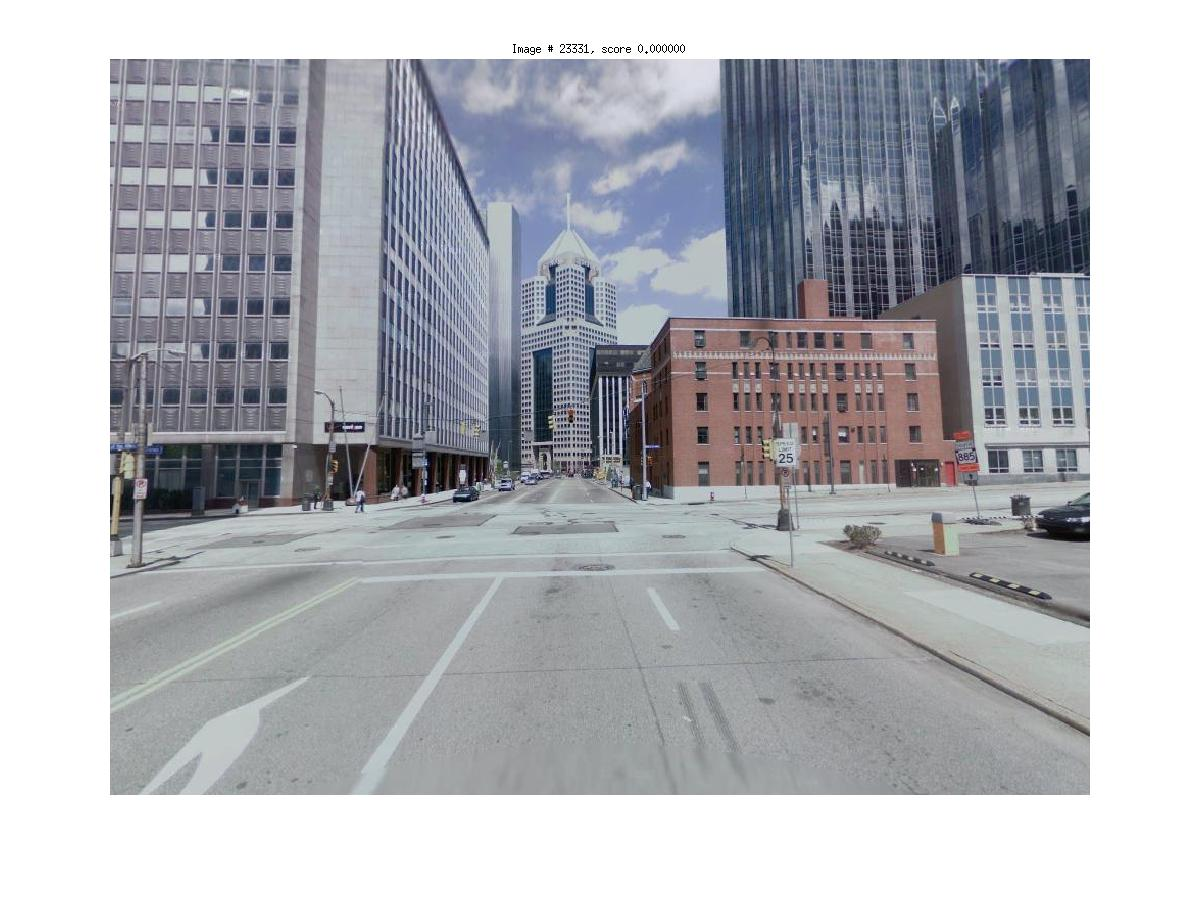
\includegraphics[trim = 35mm 30mm 35mm 30mm, clip=true, height=16mm]{imgs/Wnorm/exImproved05/improved04.jpg}}
            \end{minipage} 
        \end{minipage}
        \vspace{3mm}
        \\
        %%%%%%%%%%% Example 3 %%%%%%%%%%%%%%%
        \begin{minipage}{0.34\linewidth}
            \centering
            \vspace{0mm}
            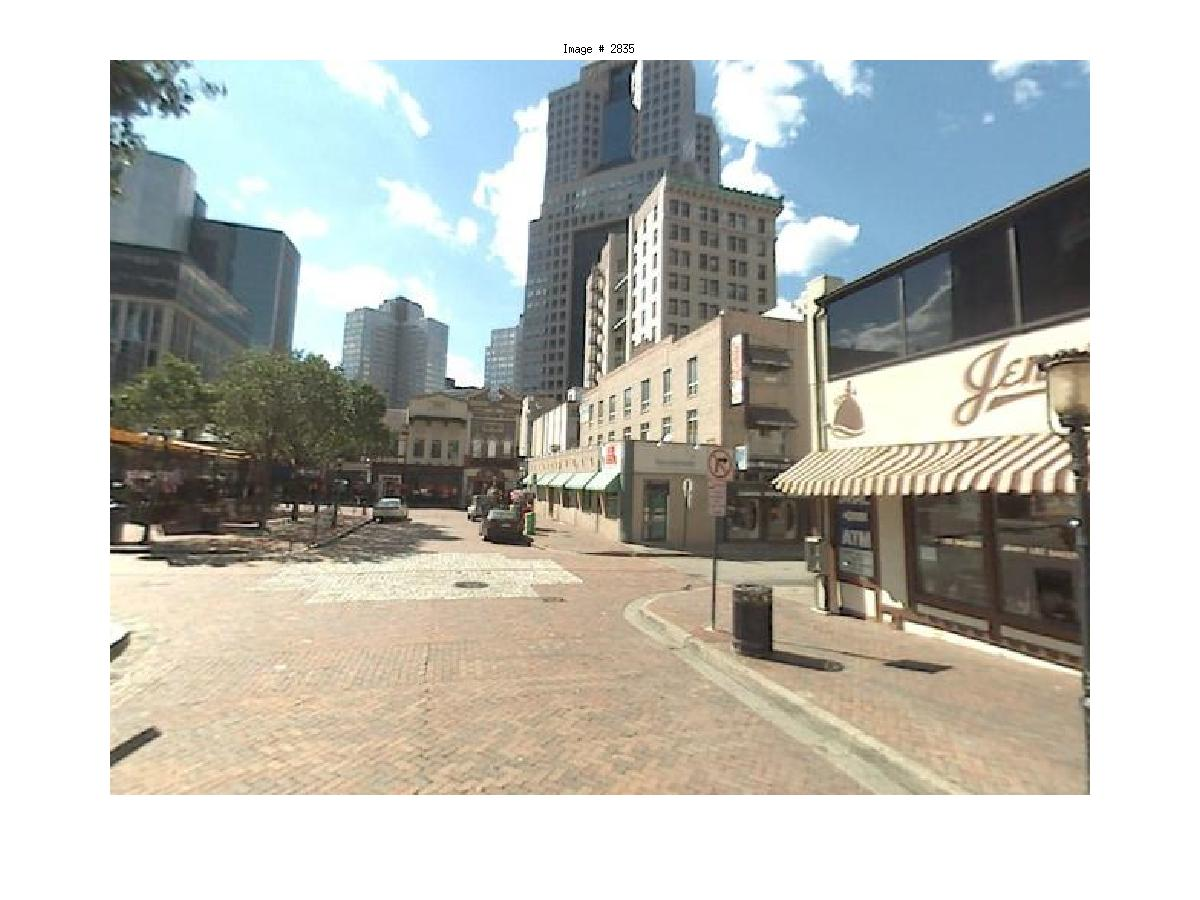
\includegraphics[trim = 45mm 40mm 45mm 30mm, clip=true, height=36mm]{imgs/Wnorm/exImproved04/query.jpg}
        \end{minipage}
        % Retrieved images
        \begin{minipage}{0.75\linewidth}
            % FV e-SVM
            \begin{minipage}{\linewidth} 
                \colorbox{myGreen}{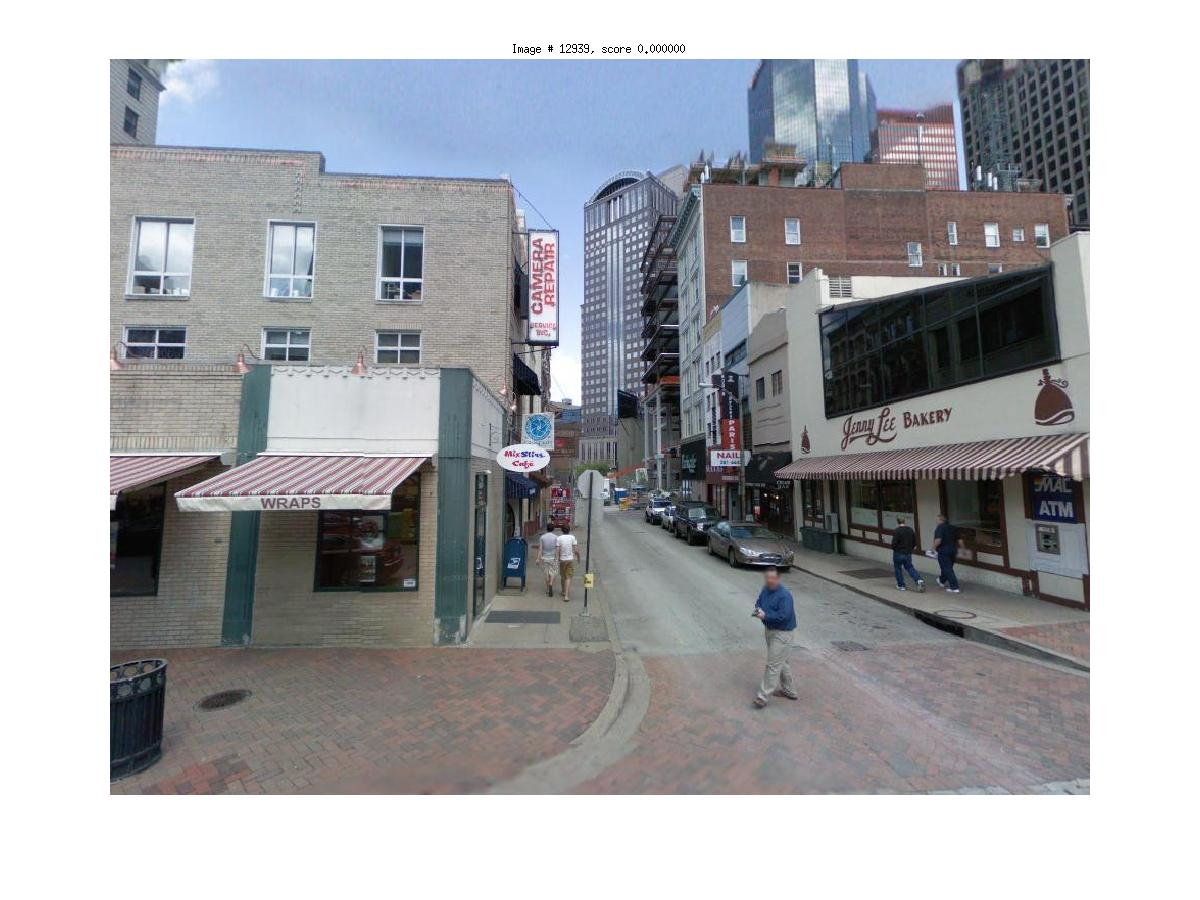
\includegraphics[trim = 35mm 30mm 35mm 30mm, clip=true, height=16mm]{imgs/Wnorm/exImproved04/improvedPval01.jpg}}
                \colorbox{myGreen}{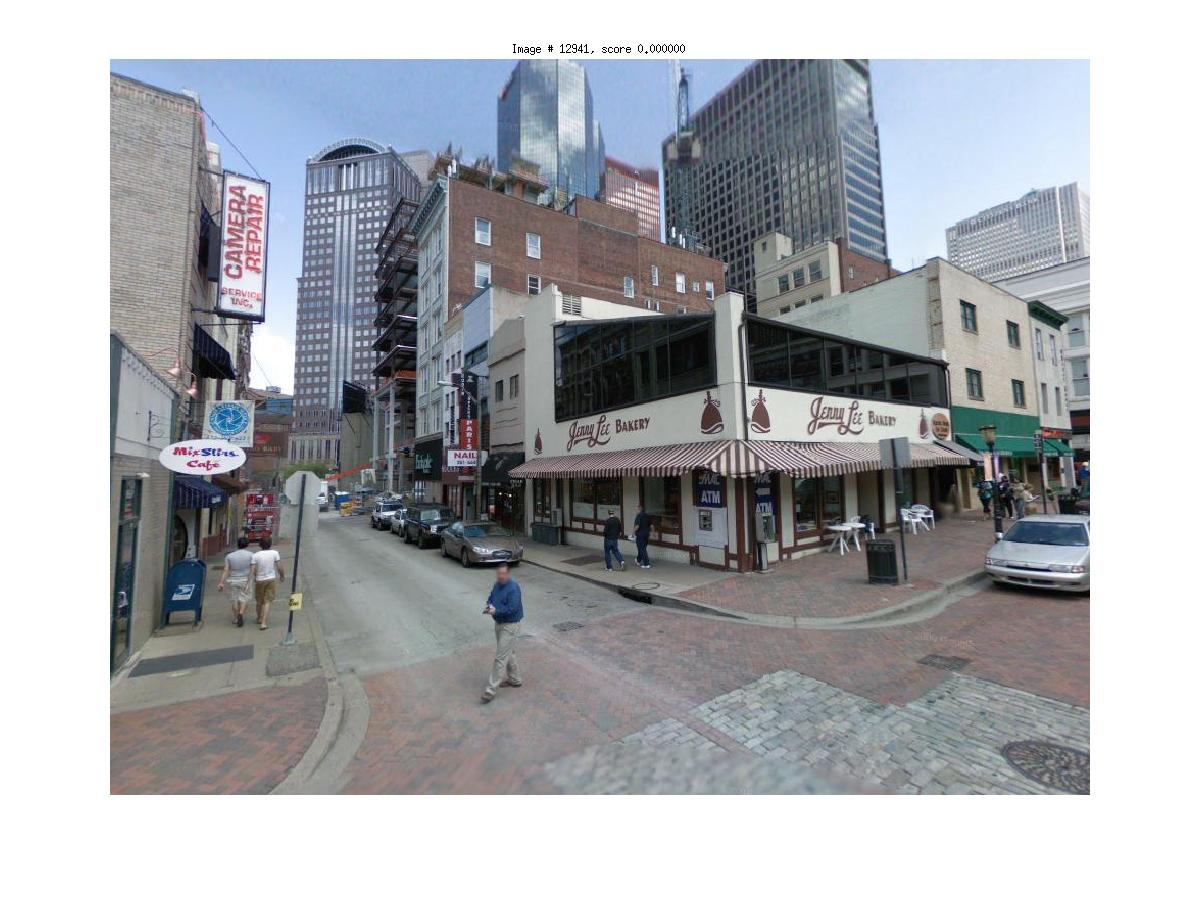
\includegraphics[trim = 35mm 30mm 35mm 30mm, clip=true, height=16mm]{imgs/Wnorm/exImproved04/improvedPval02.jpg}}
                \colorbox{myGreen}{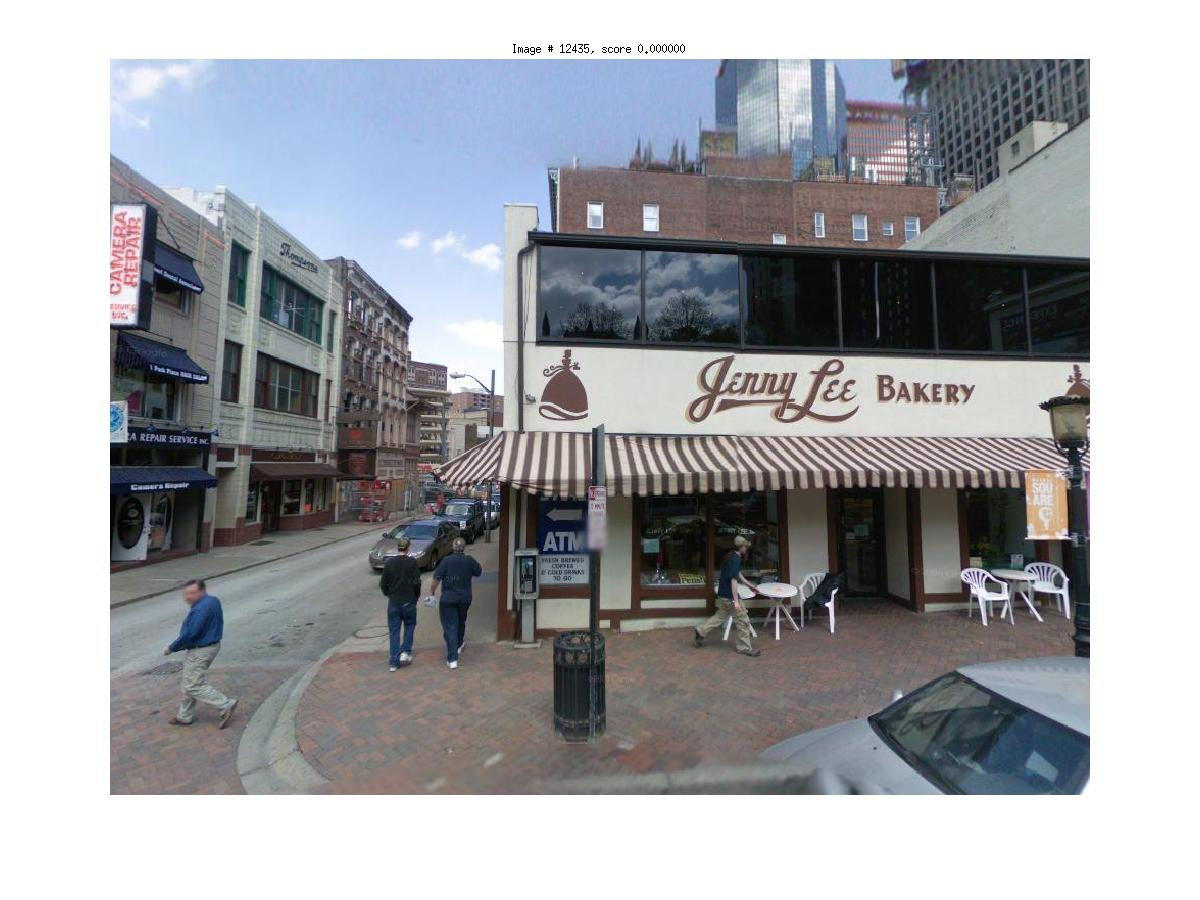
\includegraphics[trim = 35mm 30mm 35mm 30mm, clip=true, height=16mm]{imgs/Wnorm/exImproved04/improvedPval03.jpg}}
                \colorbox{myGreen}{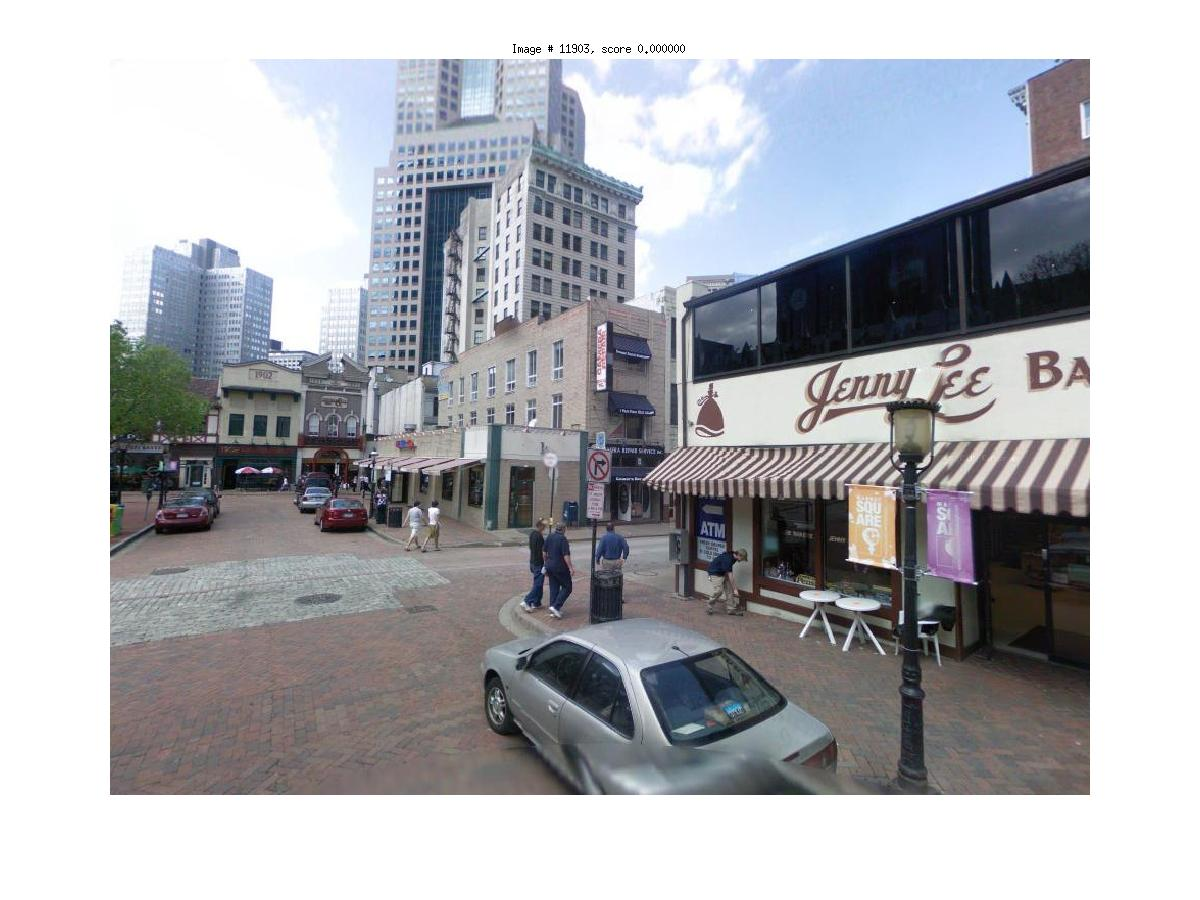
\includegraphics[trim = 35mm 30mm 35mm 30mm, clip=true, height=16mm]{imgs/Wnorm/exImproved04/improvedPval04.jpg}}
            \end{minipage}
            \\
            \begin{minipage}{\linewidth}
                \colorbox{myRed}{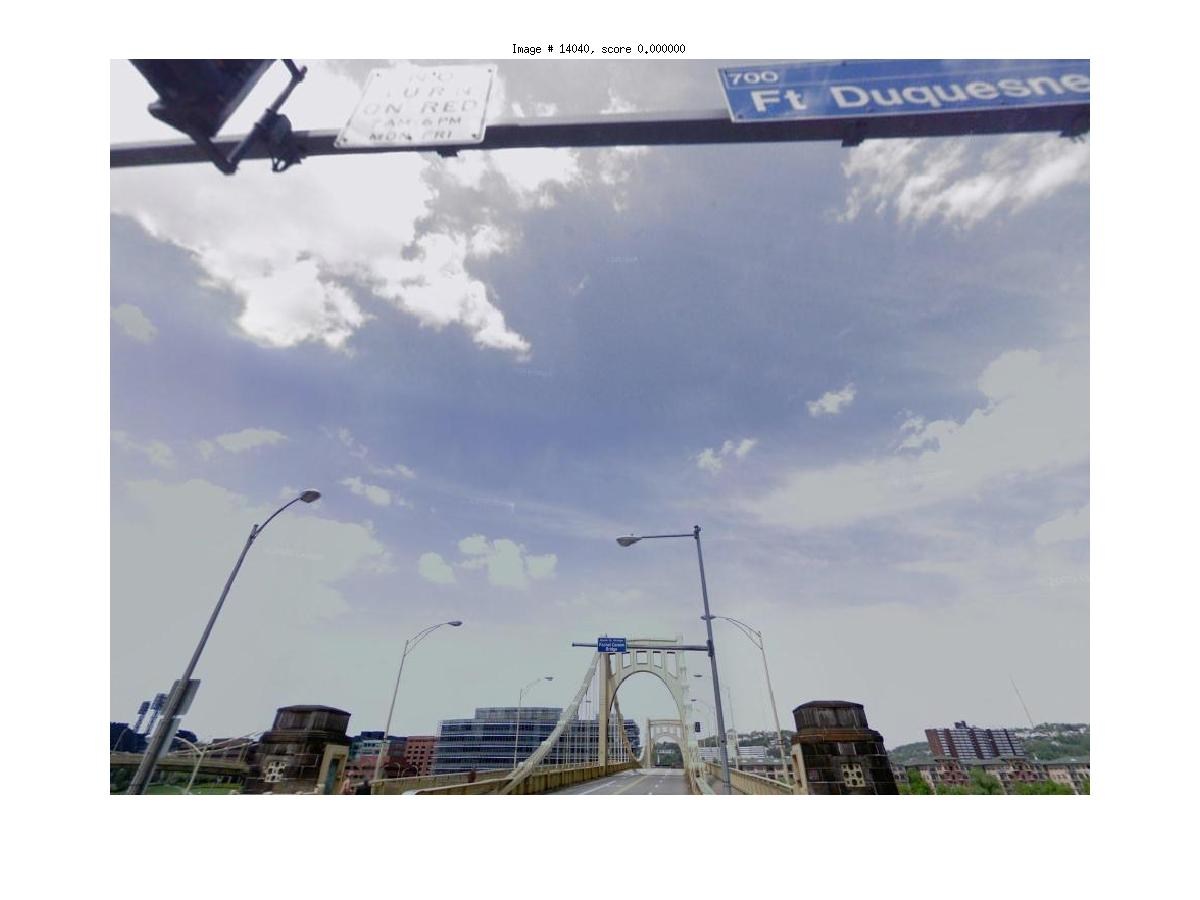
\includegraphics[trim = 35mm 30mm 35mm 30mm, clip=true, height=16mm]{imgs/Wnorm/exImproved04/improved01.jpg}}
                \colorbox{myRed}{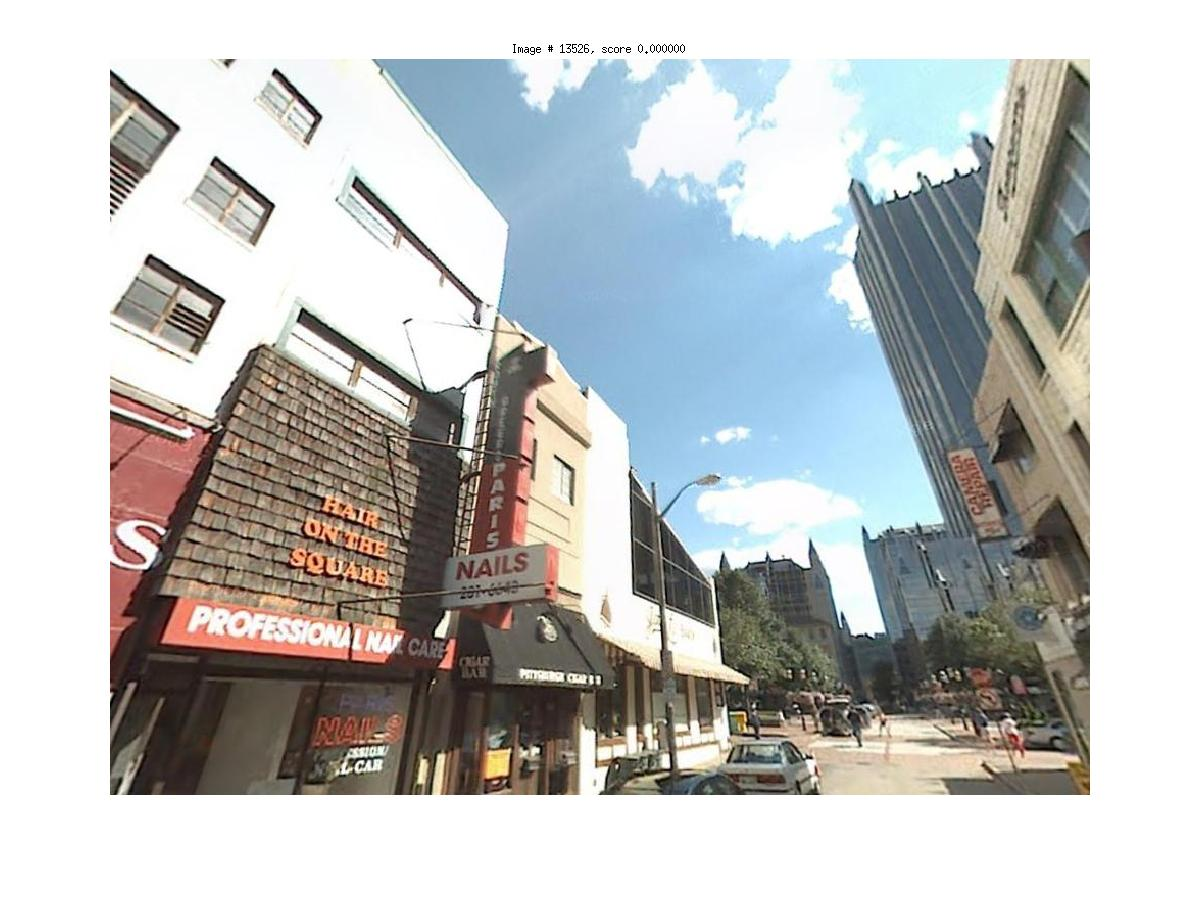
\includegraphics[trim = 35mm 30mm 35mm 30mm, clip=true, height=16mm]{imgs/Wnorm/exImproved04/improved02.jpg}}
                \colorbox{myRed}{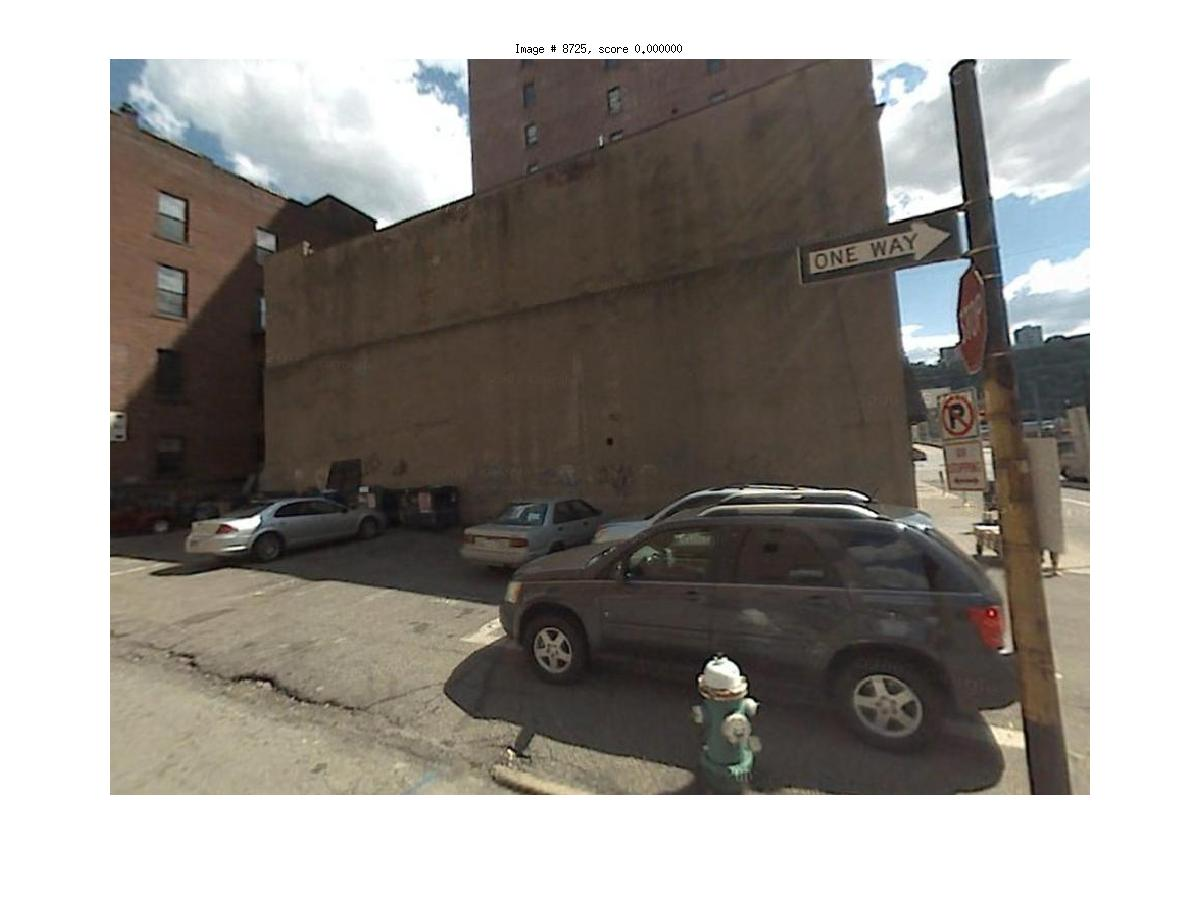
\includegraphics[trim = 35mm 30mm 35mm 30mm, clip=true, height=16mm]{imgs/Wnorm/exImproved04/improved03.jpg}}
                \colorbox{myRed}{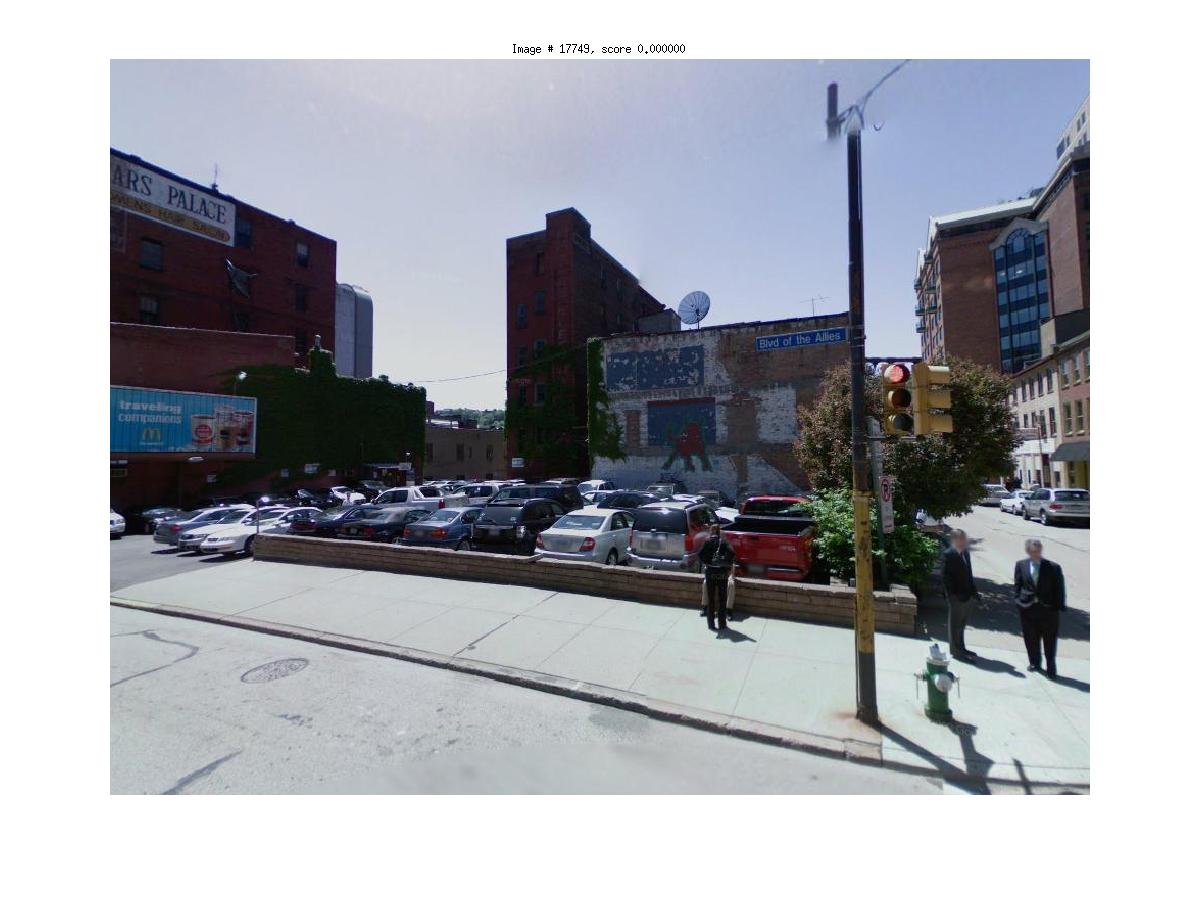
\includegraphics[trim = 35mm 30mm 35mm 30mm, clip=true, height=16mm]{imgs/Wnorm/exImproved04/improved04.jpg}}
            \end{minipage} 
        \end{minipage}
        \vspace{3mm}
        \\
        %%%%%%%%%%% MIX FAILURE CASES: good examples are Mix09 14 17 16 20
        %%%%%%%%%%% Example 4 %%%%%%%%%%%%%%%
        \begin{minipage}{0.34\linewidth}
            \centering
            \vspace{0mm}
            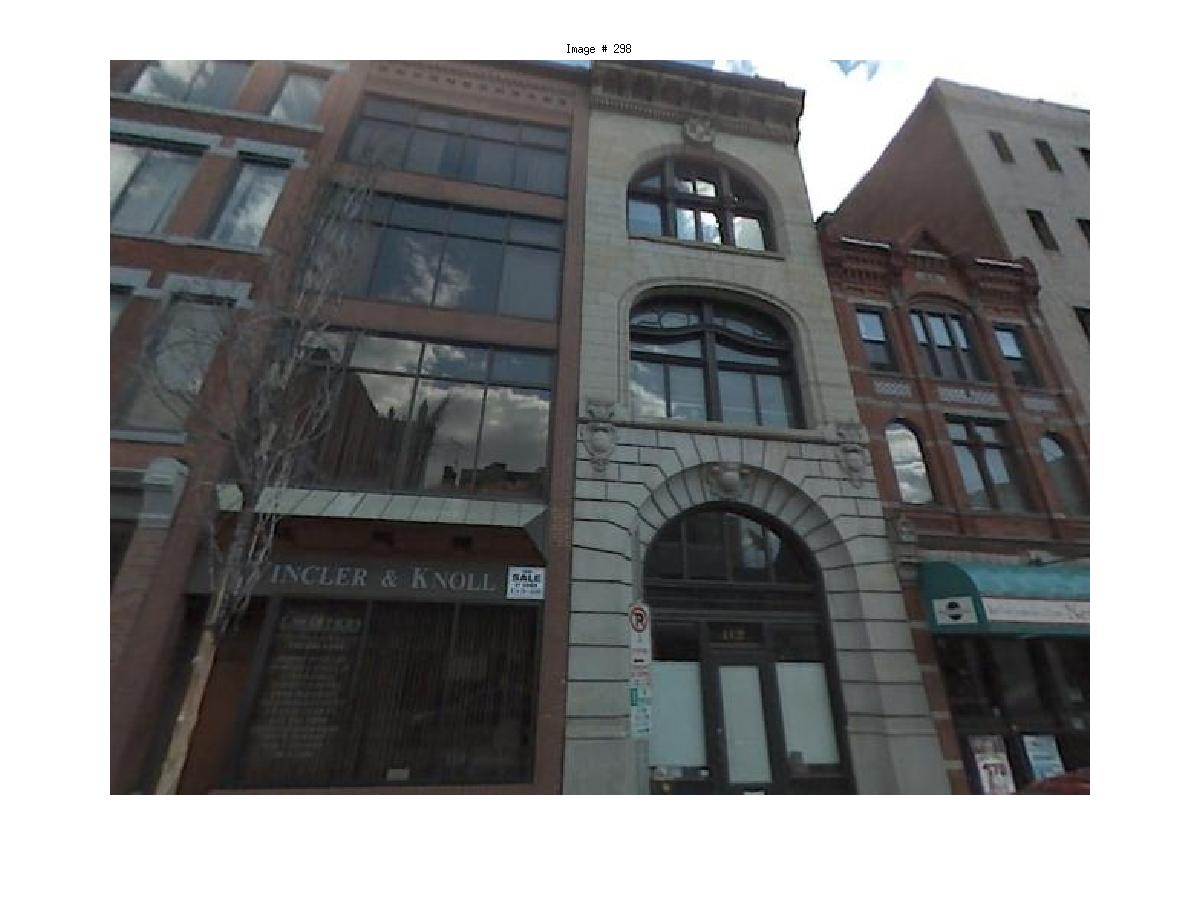
\includegraphics[trim = 45mm 40mm 45mm 30mm, clip=true, height=36mm]{imgs/Wnorm/exMix15/query.jpg}
        \end{minipage}
        % Retrieved images
        \begin{minipage}{0.75\linewidth}
            % FV e-SVM
            \begin{minipage}{\linewidth} 
                \colorbox{myRed}{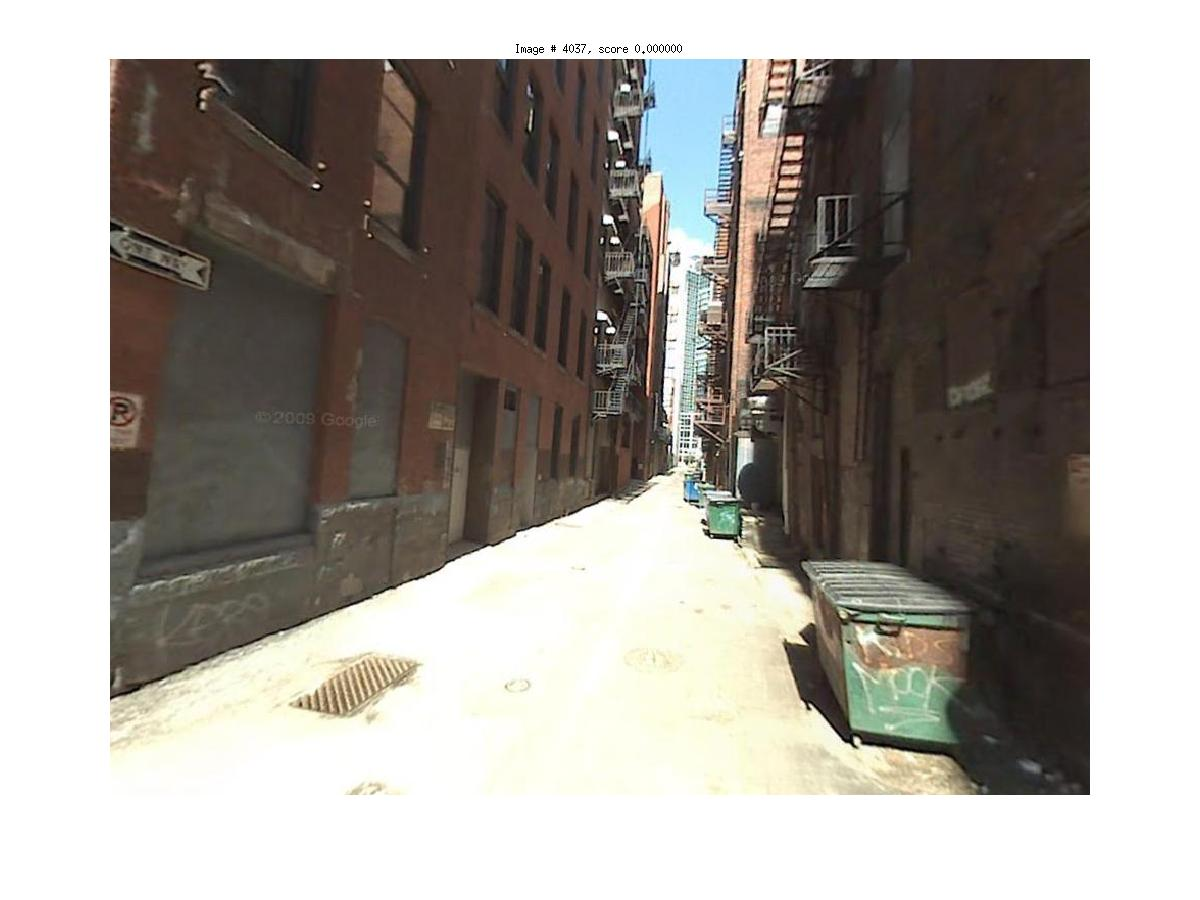
\includegraphics[trim = 35mm 30mm 35mm 30mm, clip=true, height=16mm]{imgs/Wnorm/exMix15/mixPval01.jpg}}
                \colorbox{myRed}{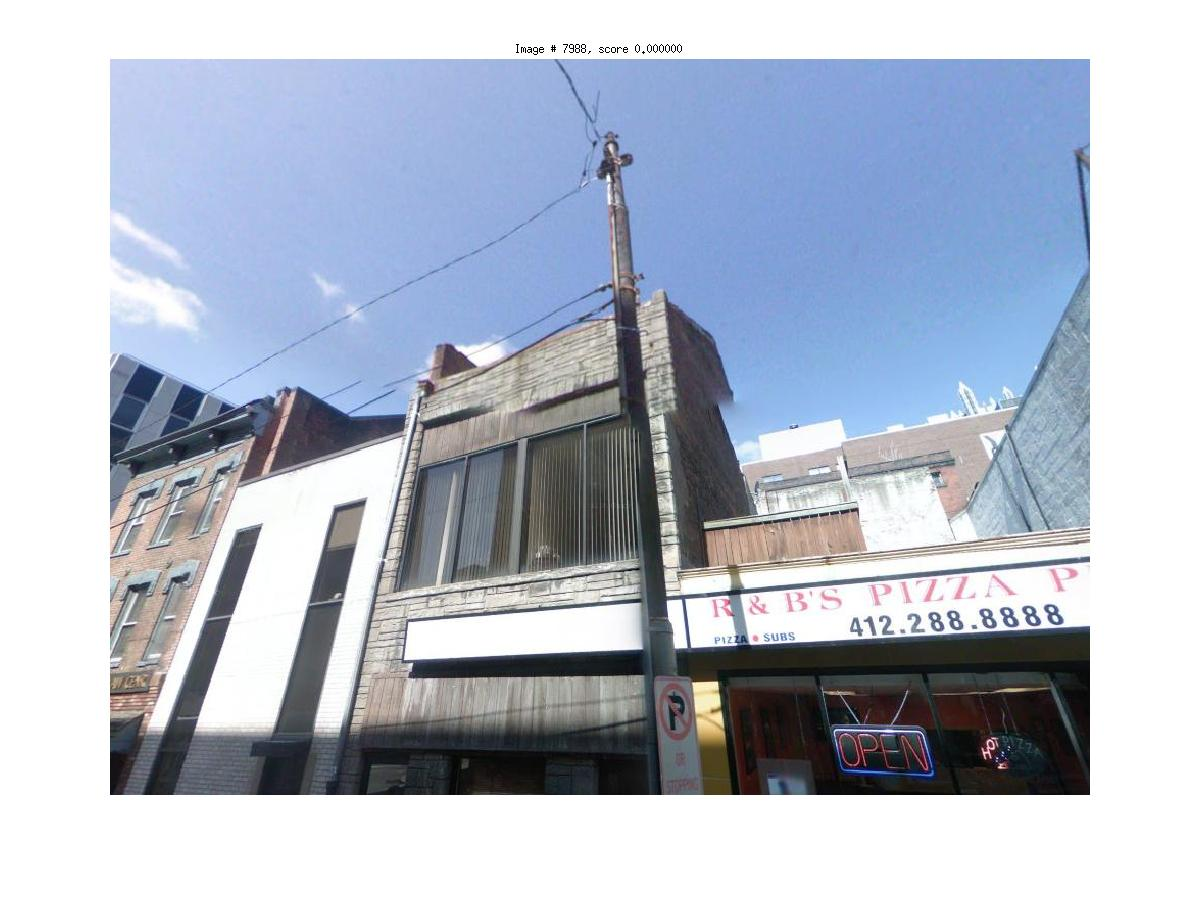
\includegraphics[trim = 35mm 30mm 35mm 30mm, clip=true, height=16mm]{imgs/Wnorm/exMix15/mixPval02.jpg}}
                \colorbox{myGreen}{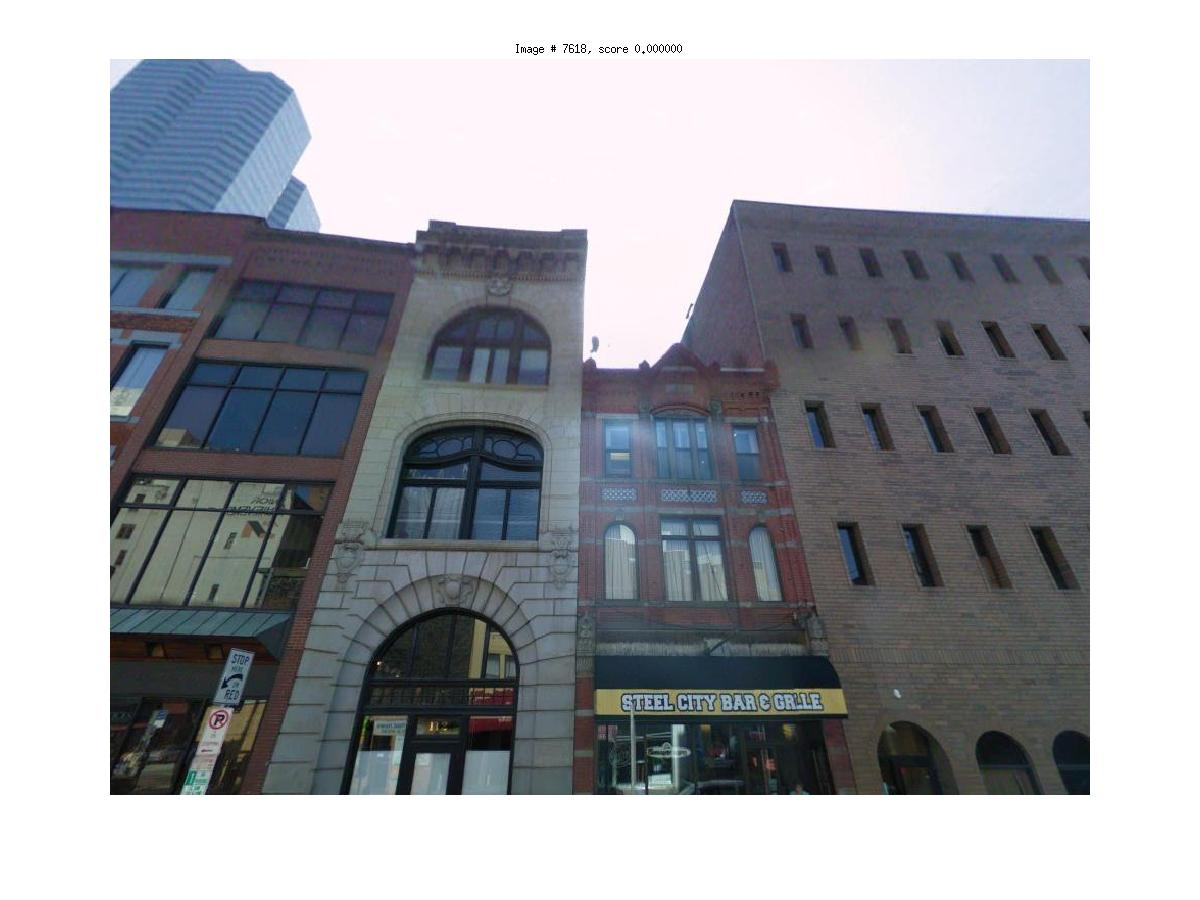
\includegraphics[trim = 35mm 30mm 35mm 30mm, clip=true, height=16mm]{imgs/Wnorm/exMix15/mixPval03.jpg}}
                \colorbox{myGreen}{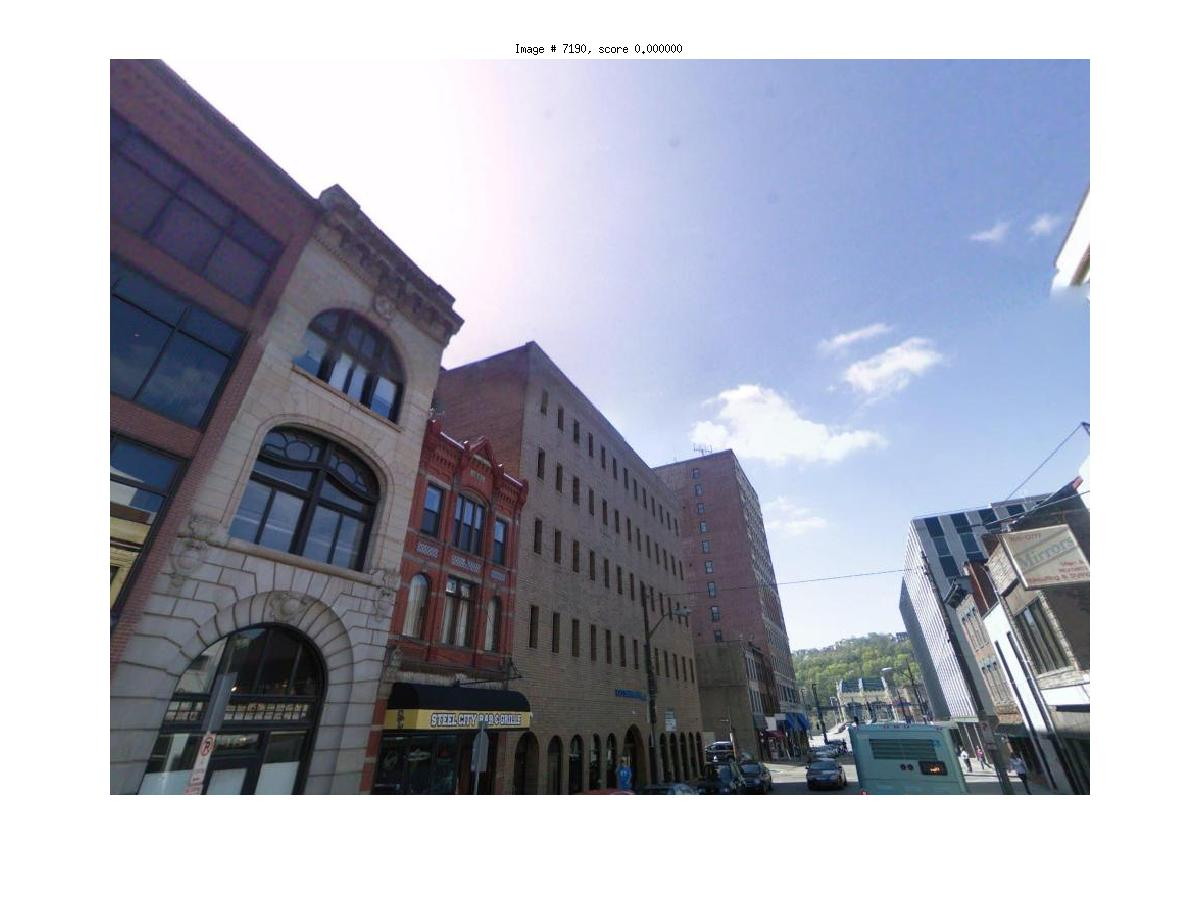
\includegraphics[trim = 35mm 30mm 35mm 30mm, clip=true, height=16mm]{imgs/Wnorm/exMix15/mixPval04.jpg}}
            \end{minipage}
            \\
            \begin{minipage}{\linewidth}
                \colorbox{myRed}{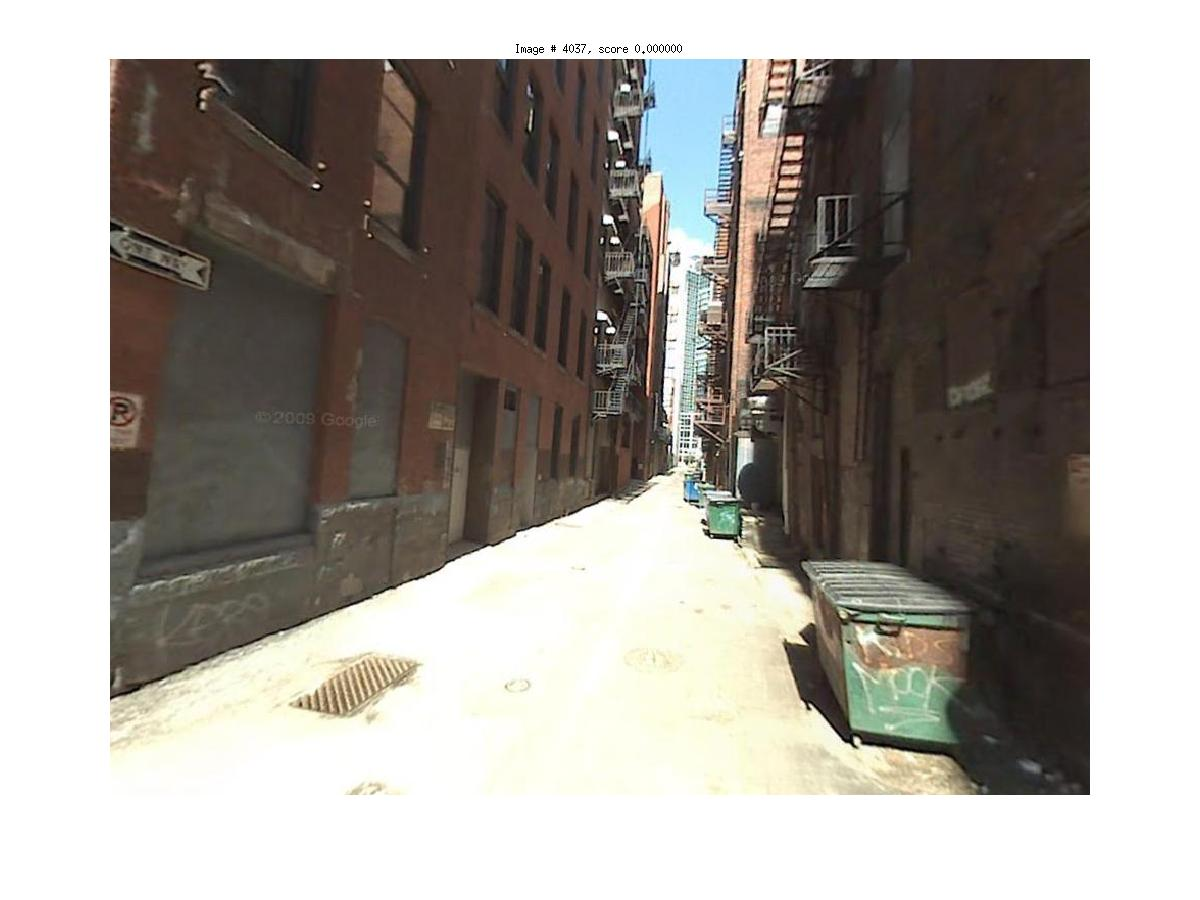
\includegraphics[trim = 35mm 30mm 35mm 30mm, clip=true, height=16mm]{imgs/Wnorm/exMix15/mix01.jpg}}
                \colorbox{myRed}{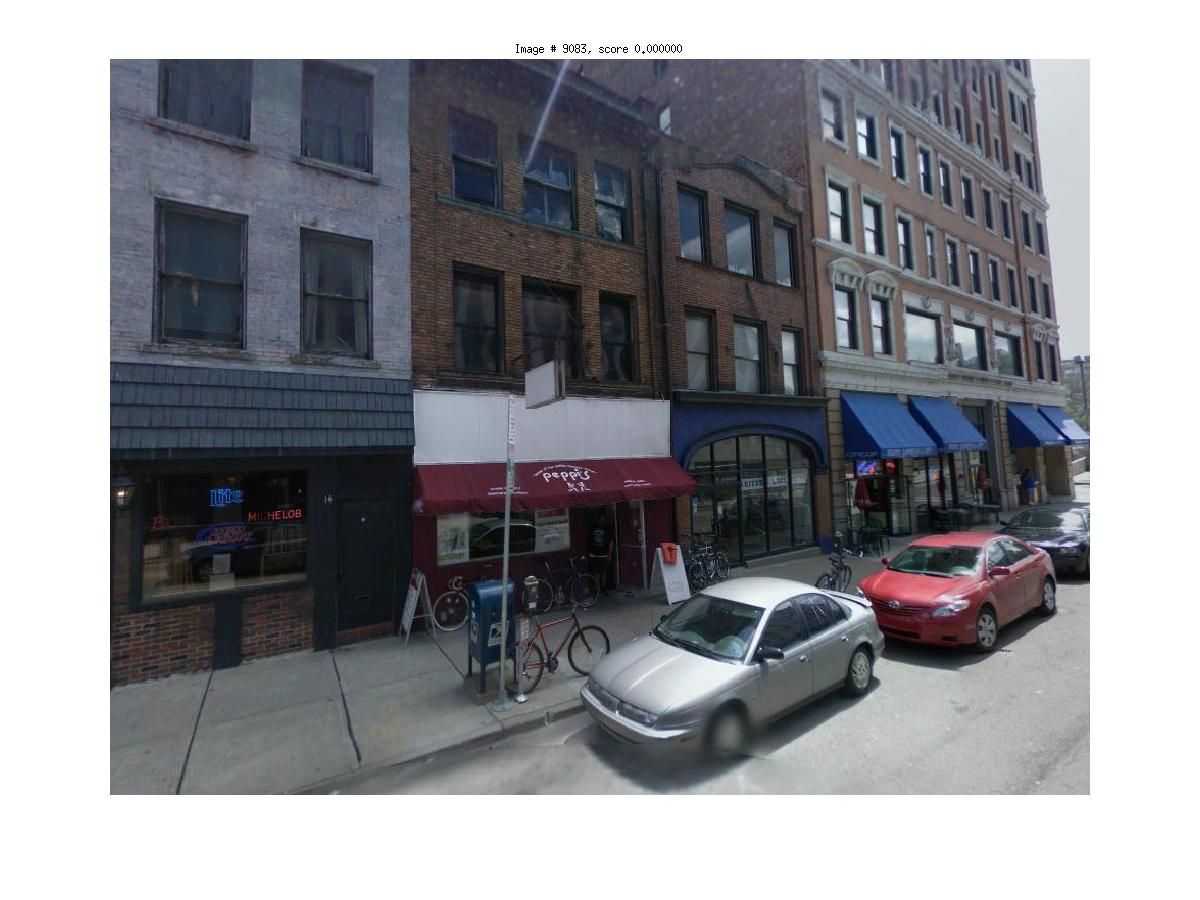
\includegraphics[trim = 35mm 30mm 35mm 30mm, clip=true, height=16mm]{imgs/Wnorm/exMix15/mix02.jpg}}
                \colorbox{myRed}{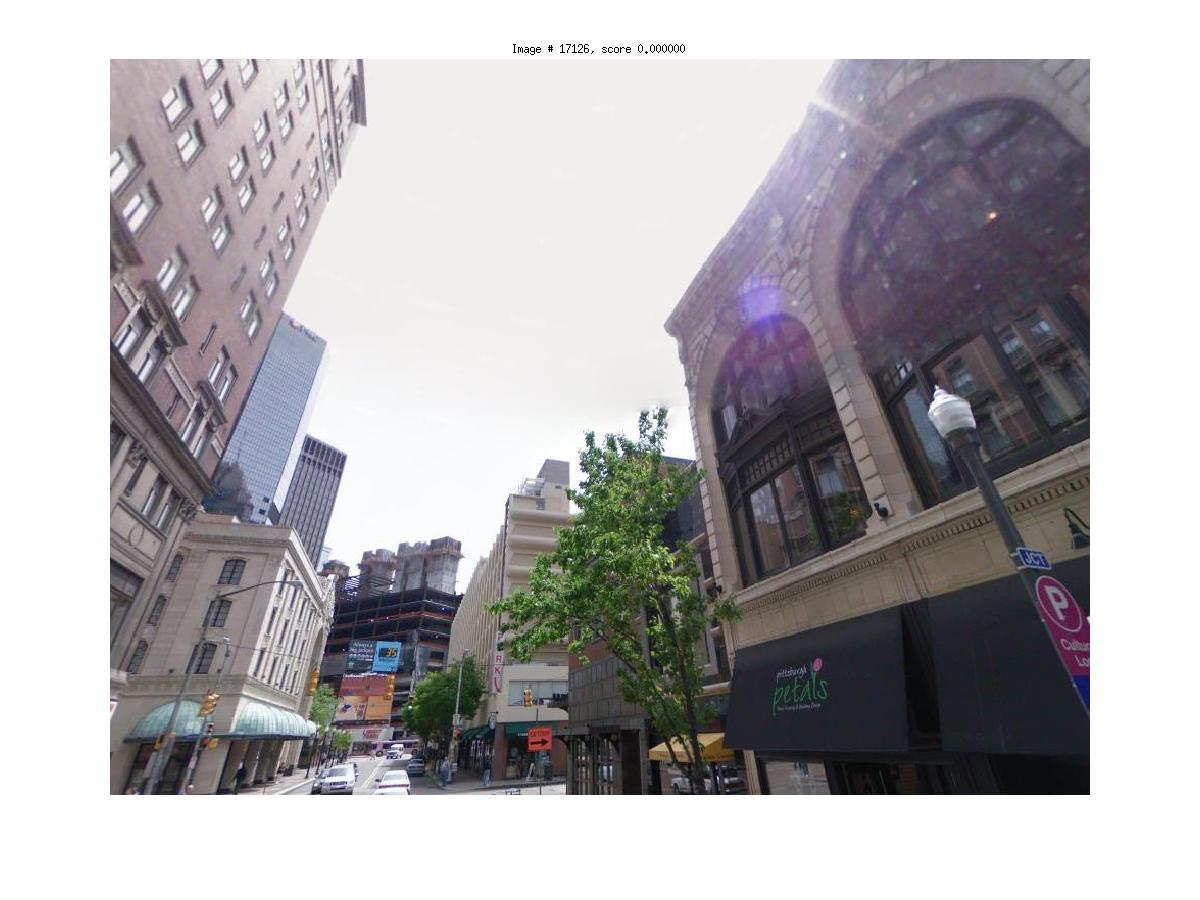
\includegraphics[trim = 35mm 30mm 35mm 30mm, clip=true, height=16mm]{imgs/Wnorm/exMix15/mix03.jpg}}
                \colorbox{myGreen}{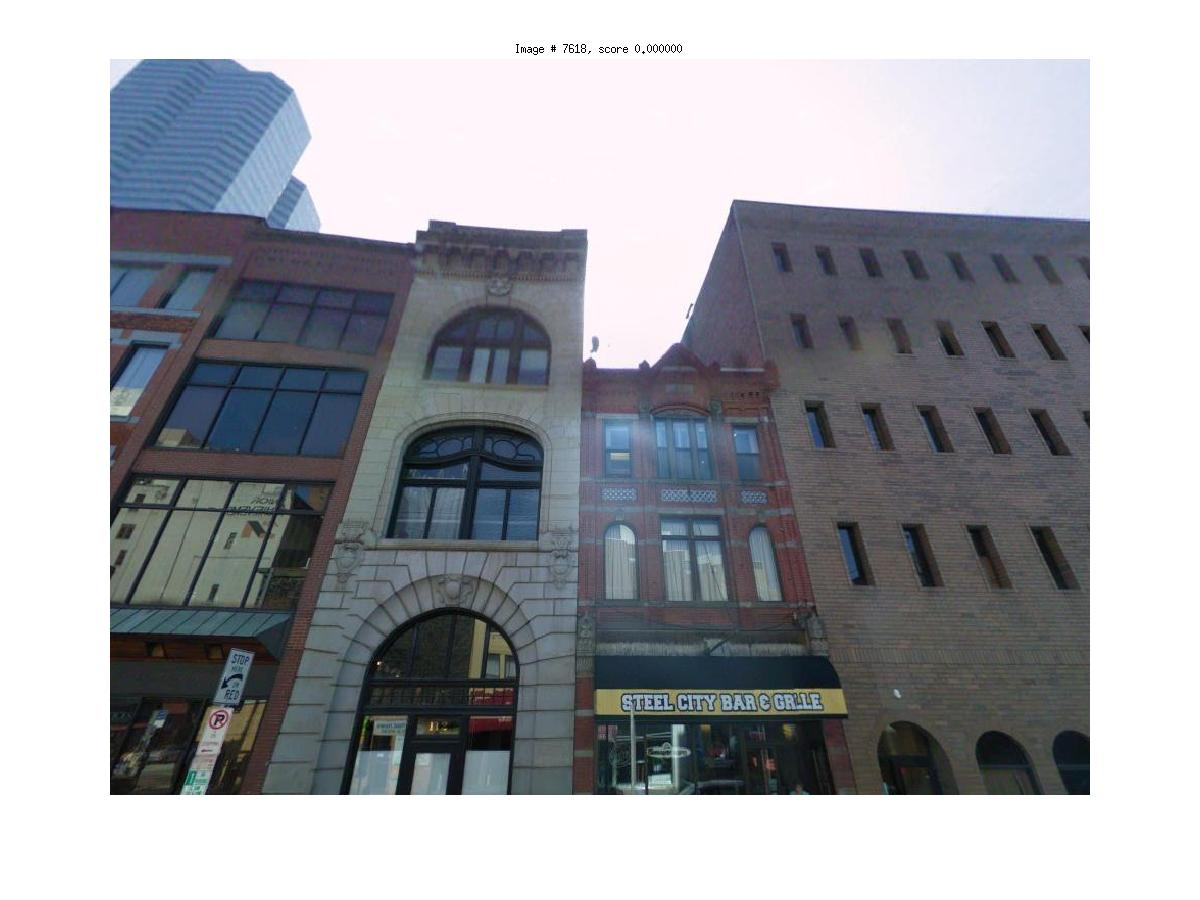
\includegraphics[trim = 35mm 30mm 35mm 30mm, clip=true, height=16mm]{imgs/Wnorm/exMix15/mix04.jpg}}
            \end{minipage} 
        \end{minipage}
        \vspace{3mm}
        \\
        %%%%%%%%%%% Example 5 %%%%%%%%%%%%%%%
        \begin{minipage}{0.34\linewidth}
            \centering
            \vspace{0mm}
            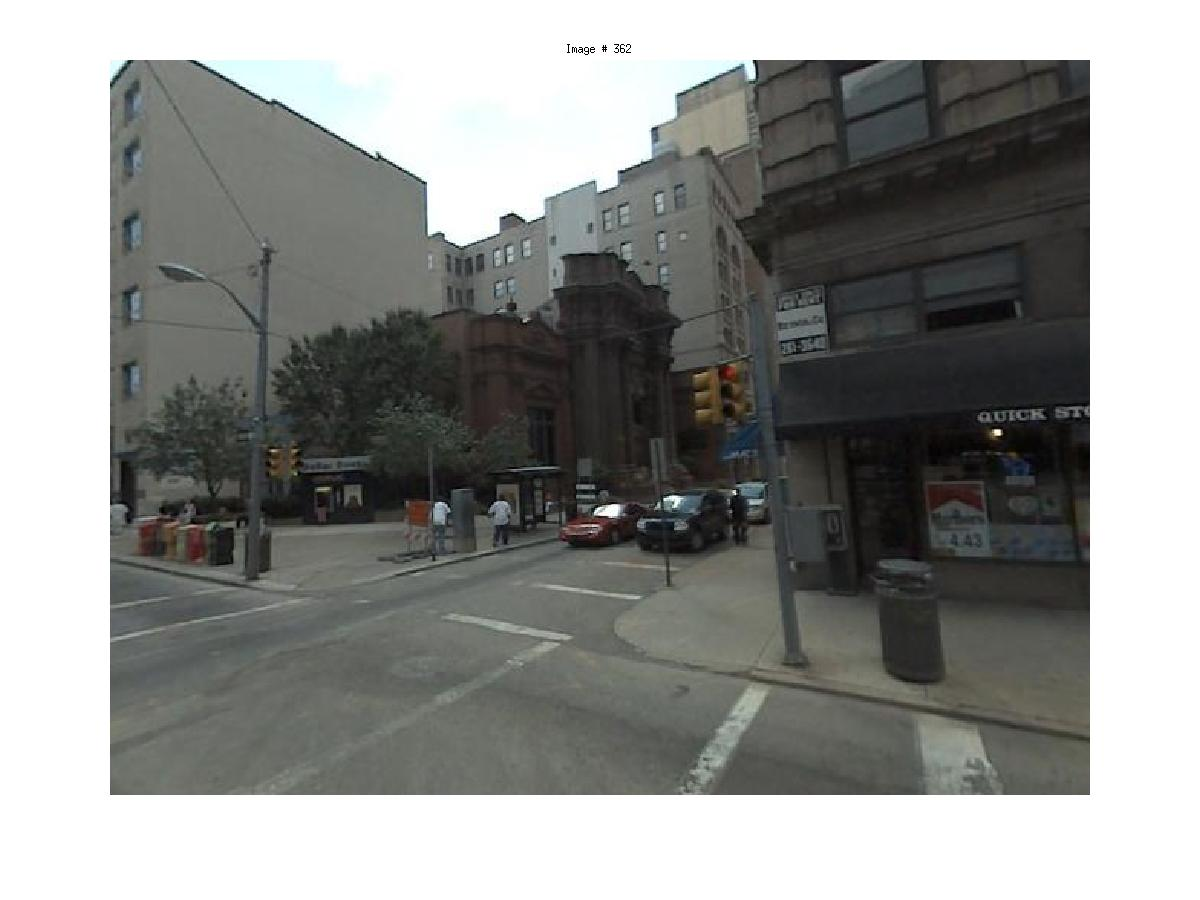
\includegraphics[trim = 45mm 40mm 45mm 30mm, clip=true, height=36mm]{imgs/Wnorm/exMix19/query.jpg}
        \end{minipage}
        % Retrieved images
        \begin{minipage}{0.75\linewidth}
            % FV e-SVM
            \begin{minipage}{\linewidth} 
                \colorbox{myGreen}{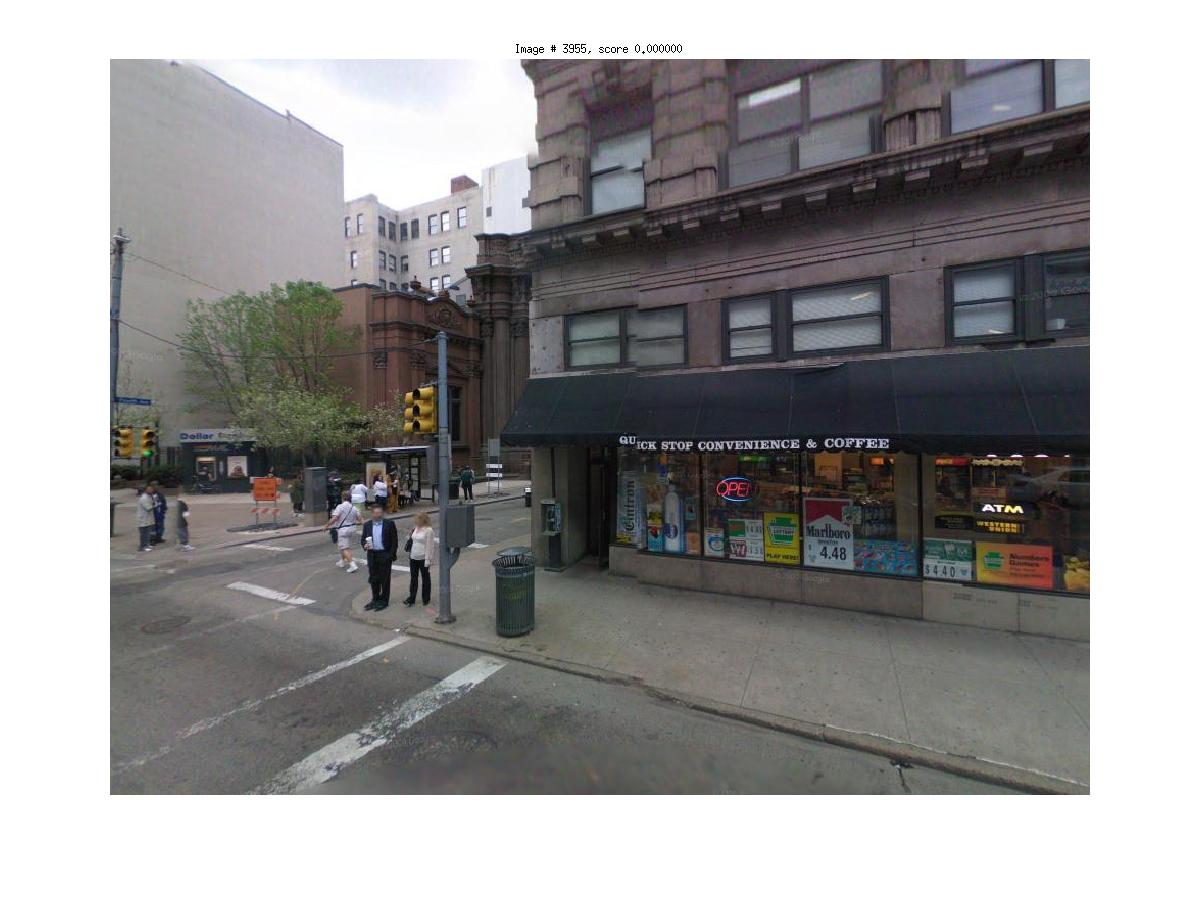
\includegraphics[trim = 35mm 30mm 35mm 30mm, clip=true, height=16mm]{imgs/Wnorm/exMix19/mixPval01.jpg}}
                \colorbox{myRed}{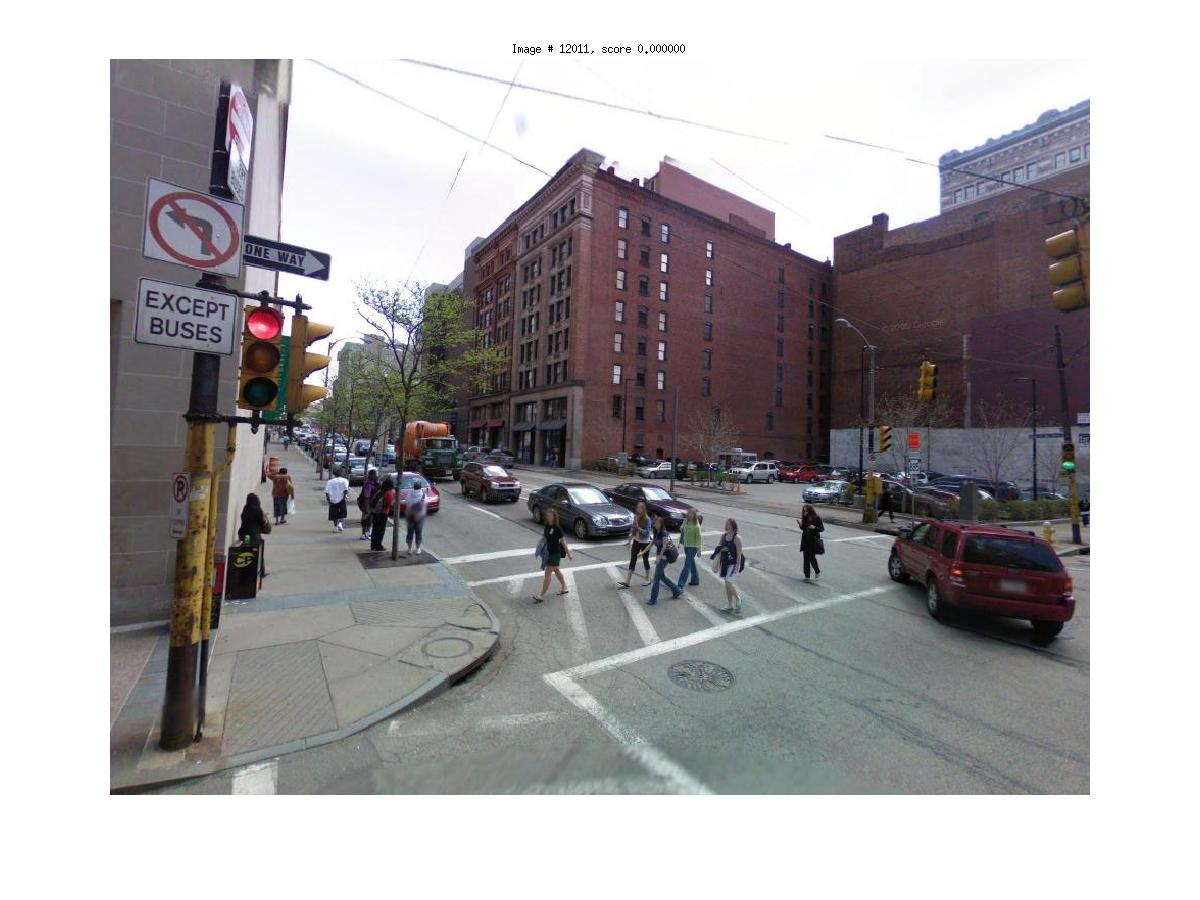
\includegraphics[trim = 35mm 30mm 35mm 30mm, clip=true, height=16mm]{imgs/Wnorm/exMix19/mixPval02.jpg}}
                \colorbox{myGreen}{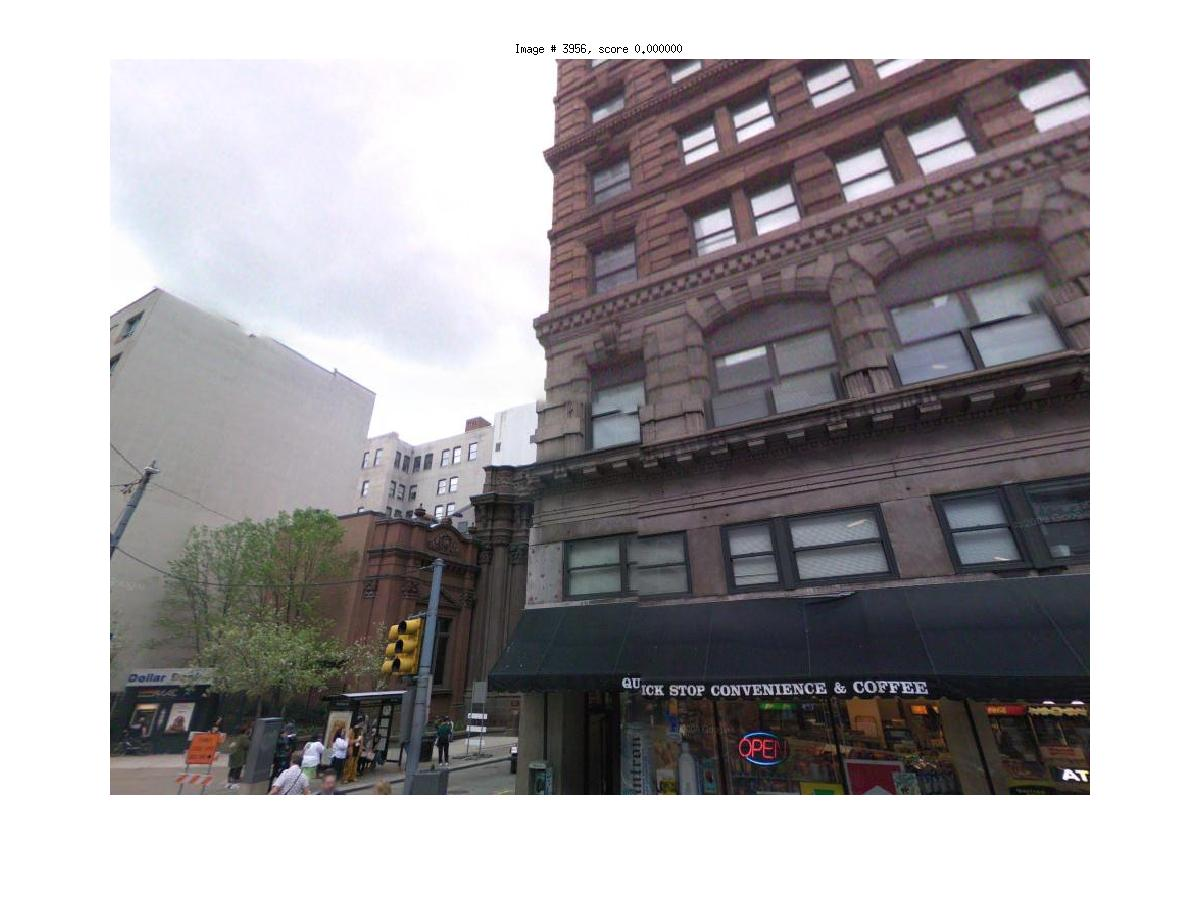
\includegraphics[trim = 35mm 30mm 35mm 30mm, clip=true, height=16mm]{imgs/Wnorm/exMix19/mixPval03.jpg}}
                \colorbox{myGreen}{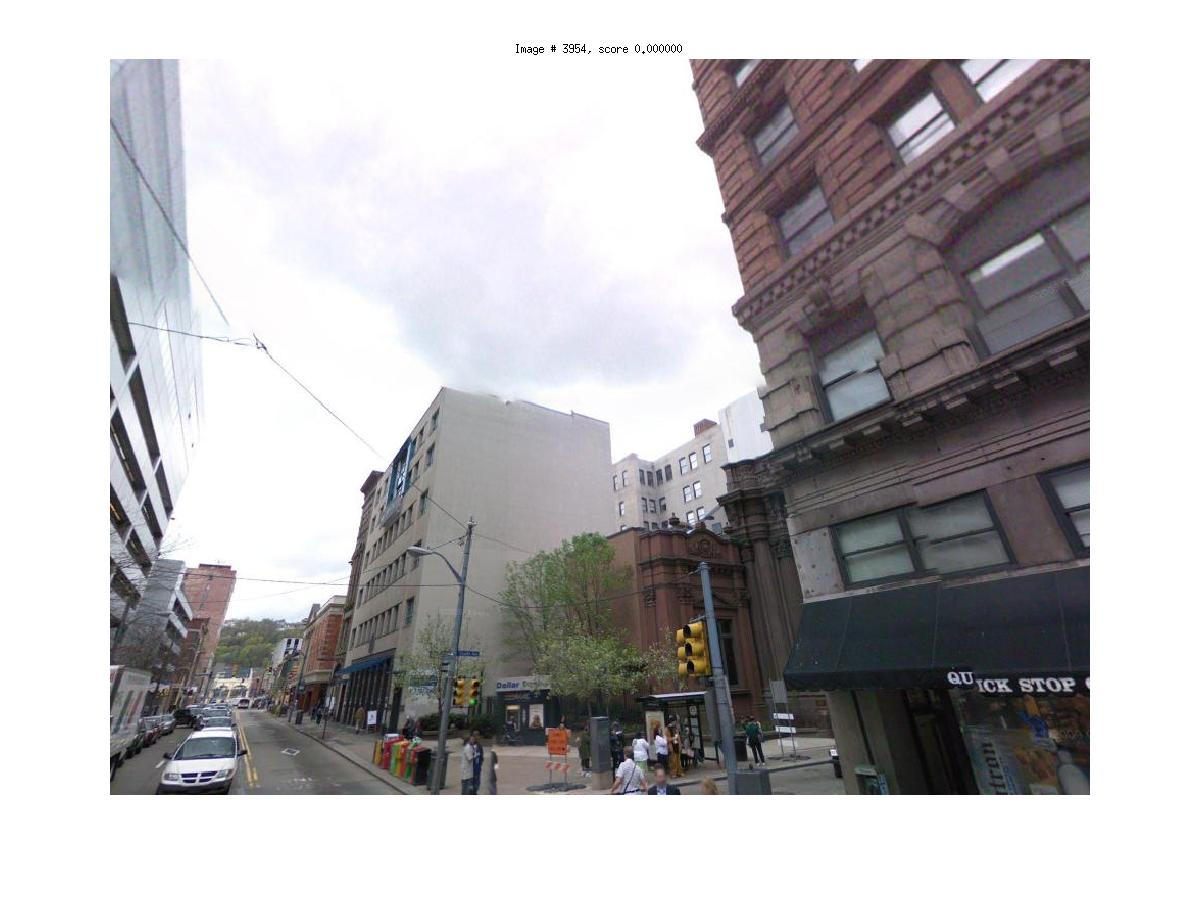
\includegraphics[trim = 35mm 30mm 35mm 30mm, clip=true, height=16mm]{imgs/Wnorm/exMix19/mixPval04.jpg}}
            \end{minipage}
            \\
            \begin{minipage}{\linewidth}
                \colorbox{myGreen}{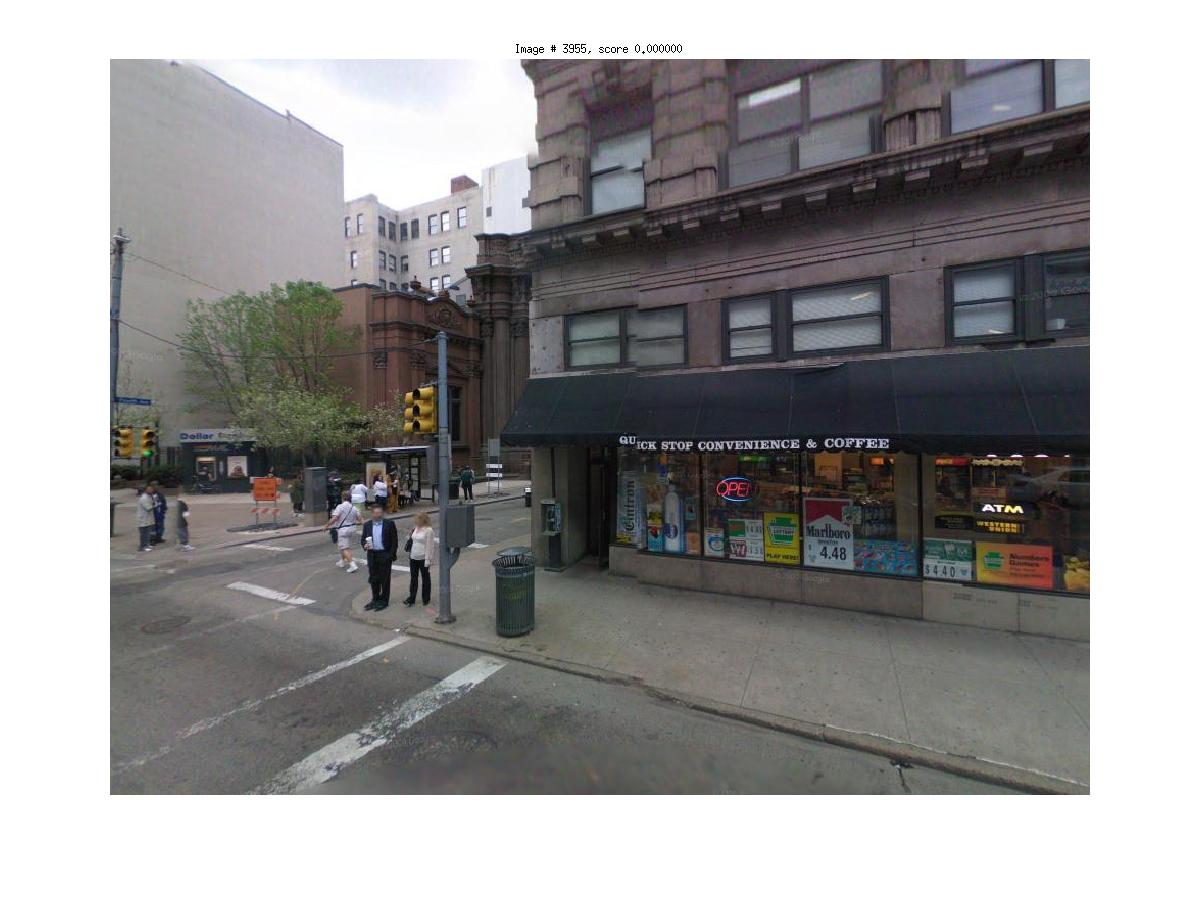
\includegraphics[trim = 35mm 30mm 35mm 30mm, clip=true, height=16mm]{imgs/Wnorm/exMix19/mix01.jpg}}
                \colorbox{myRed}{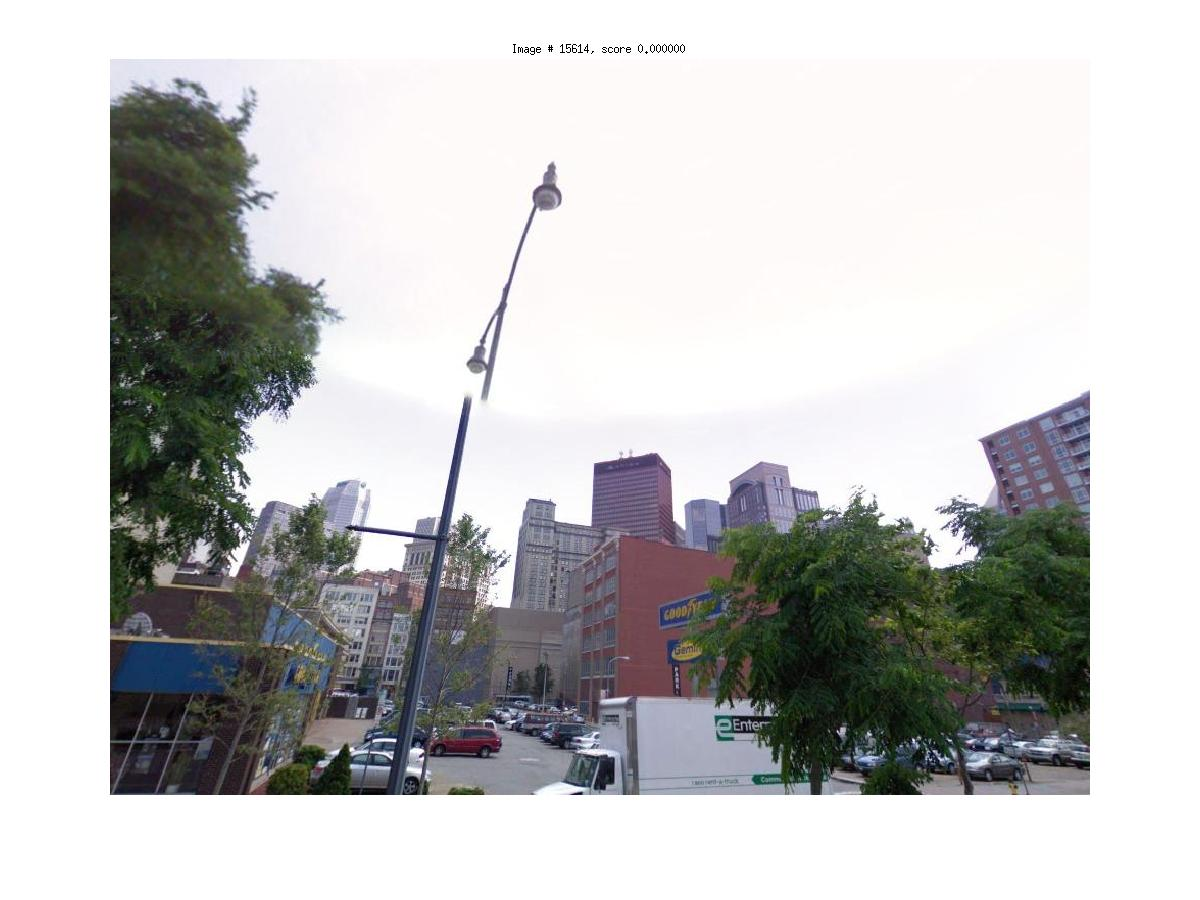
\includegraphics[trim = 35mm 30mm 35mm 30mm, clip=true, height=16mm]{imgs/Wnorm/exMix19/mix02.jpg}}
                \colorbox{myRed}{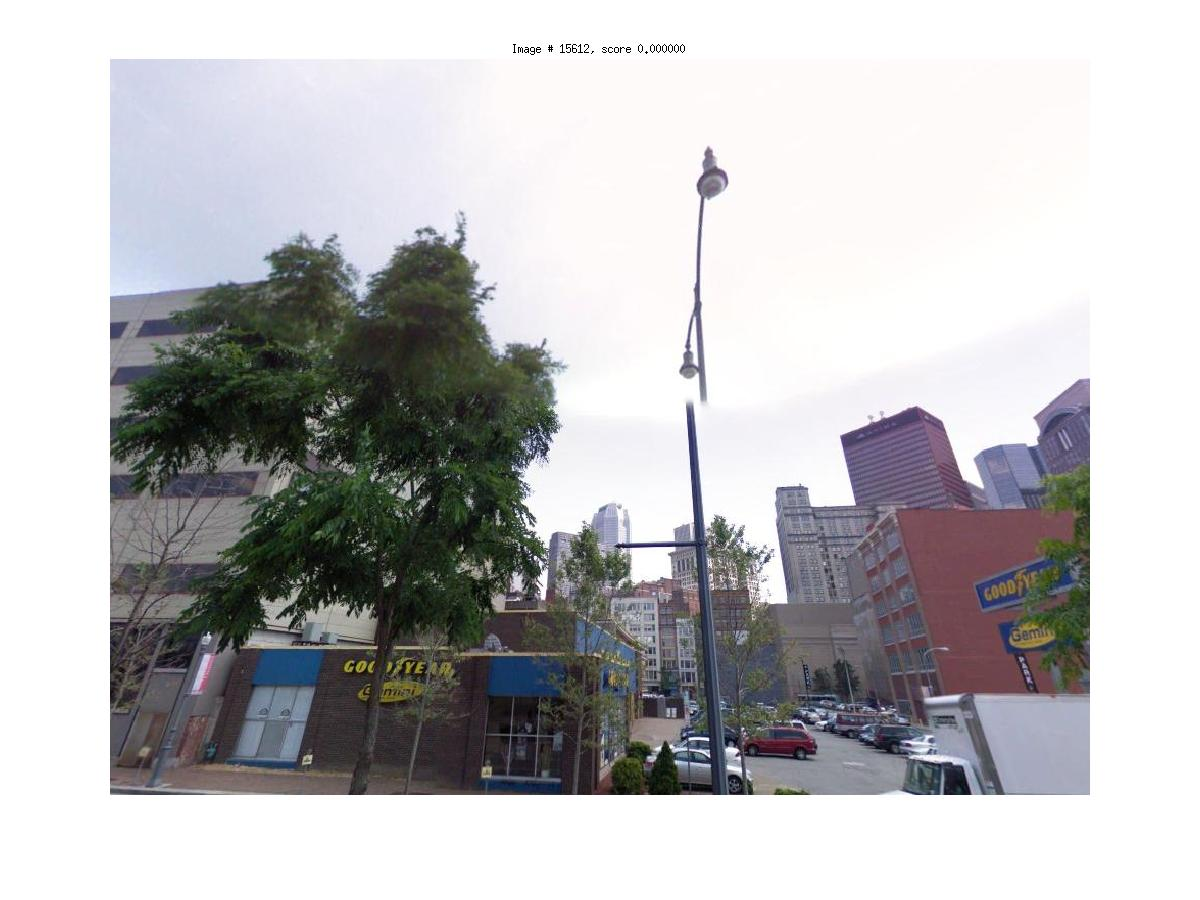
\includegraphics[trim = 35mm 30mm 35mm 30mm, clip=true, height=16mm]{imgs/Wnorm/exMix19/mix03.jpg}}
                \colorbox{myRed}{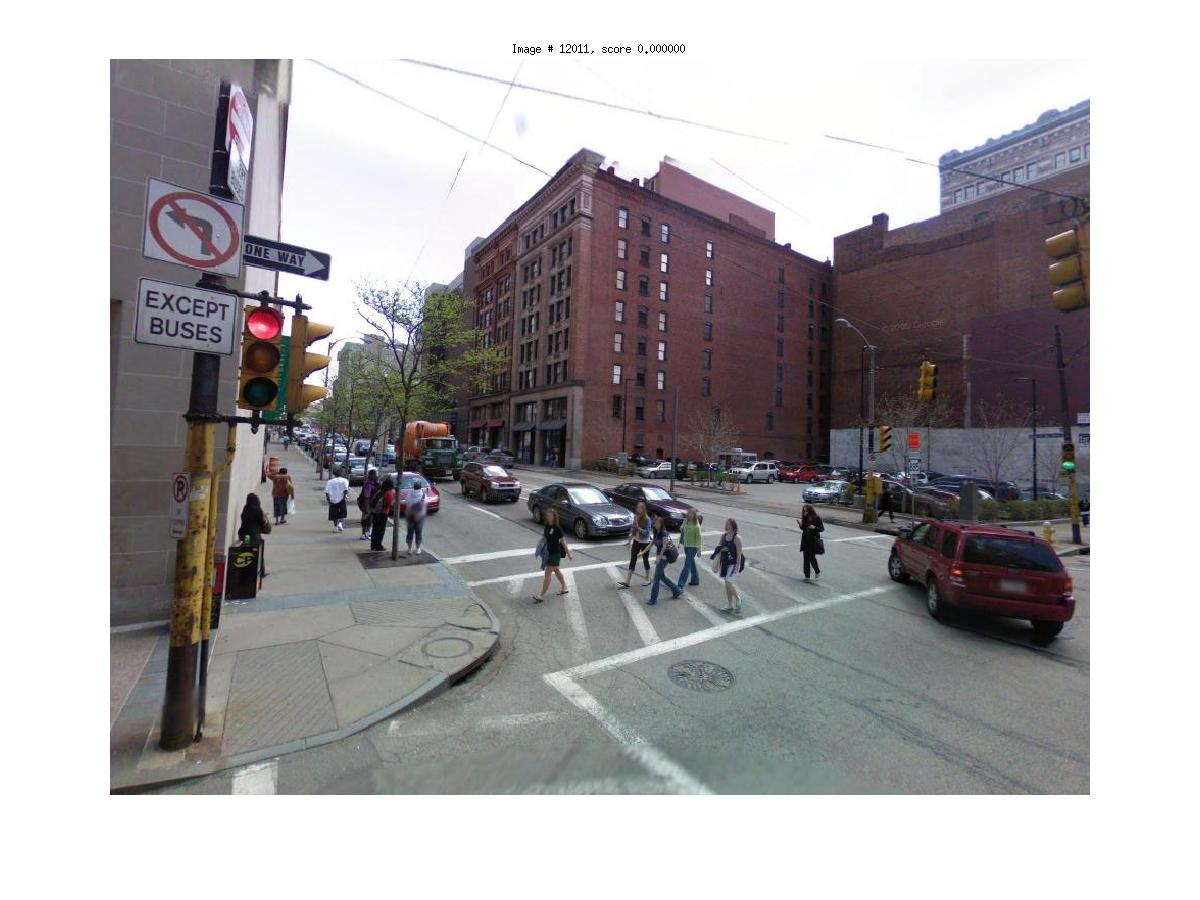
\includegraphics[trim = 35mm 30mm 35mm 30mm, clip=true, height=16mm]{imgs/Wnorm/exMix19/mix04.jpg}}
            \end{minipage} 
        \end{minipage}
        %%%%%%%%%%%%%%%%%%%%%%%%%%%%%%%%%%%%%

            \caption{
                \textbf{Examples of correctly and incorrectly localized queries for the learnt Fisher vector representation.}
                Each example shows a query image (left) together with correct (green) and incorrect (red) matches from the database obtained by the learnt Fisher vector representation \emph{e-SVM} method (top) and the standard Fisher vector baseline (bottom) for dimension 128. Note that the proposed method is able to recognize the place depicted in the query image despite changes in viewpoint, illumination and partial occlusion by other objects (trees, lamps) and buildings. 
                Note that the baseline methods often finds images depicting the same buildings but in a distance whereas our learnt representation often finds a closer view better matching the content of the query.       
            }
            \label{fig:images}
         \end{figure*}
         %
         %
         %

   \section{Conclusions}
      We have shown that a discriminative yet compact image representation for place recognition can be learnt using the exemplar support vector machine applied to Fisher vector image descriptors without the need for expensive and tedious calibration typical for other exemplar  support vector machine methods. 
      \textcolor{petr}{We demonstrate that proposed method is applicable to two different descriptors, the bag-of-visual-words and Fisher vectors.}
      Our results show significant gains in place recognition performance compared to raw Fisher vector matching as well as other baselines. Our work opens-up the possibility of learning a compact and discriminative representation using other descriptors such as HOG~\cite{Dalal05} or the recently developed convolutional neural network features~\cite{Donahue13,Krizhevsky12,Oquab14,Sermanet13} as well as extending the analysis to other cost functions~\cite{Gharbi12,Hariharan12}. 

\small{
   \bibliographystyle{ieee}
   \bibliography{shortstrings,vggroup,cvww_template,mybib}
}

\end{document}
